\ifx\master\undefined% AUTOCOMPILE
% Allows for individual chapters to be compiled.

% Usage:
% \ifx\master\undefined% AUTOCOMPILE
% Allows for individual chapters to be compiled.

% Usage:
% \ifx\master\undefined% AUTOCOMPILE
% Allows for individual chapters to be compiled.

% Usage:
% \ifx\master\undefined\input{../settings/autocompile}\fi
% (place at start and end of chapter file)

\ifx\noprelim\undefined
    % first time included
    % input preamble files
    \input{../settings/phdsetup}

    \begin{document}
    \def\noprelim{}
\else
    % already included once
    % input post files

    \singlespacing
    \bibliographystyle{../bibliography/expanded}
    \bibliography{../bibliography/references}

    \end{document}
\fi\fi
% (place at start and end of chapter file)

\ifx\noprelim\undefined
    % first time included
    % input preamble files
    % [ USER VARIABLES ]

\def\PHDTITLE {Extensions of the Theory of Computational Mechanics}
\def\PHDAUTHOR{Evan Klose Friis}
\def\PHDSCHOOL{University of California, Davis}

\def\PHDMONTH {June}
\def\PHDYEAR  {2011}
\def\PHDDEPT {Physics}

\def\BSSCHOOL {University of California at San Diego}
\def\BSYEAR   {2005}

\def\PHDCOMMITTEEA{Professor John Conway}
\def\PHDCOMMITTEEB{Professor Robin Erbacher}
\def\PHDCOMMITTEEC{Professor Mani Tripathi}

% [ GLOBAL SETUP ]

\documentclass[letterpaper,oneside,11pt]{report}

\usepackage{calc}
\usepackage{breakcites}
\usepackage[newcommands]{ragged2e}

\usepackage[pdftex]{graphicx}
\usepackage{epstopdf}

%\usepackage{tikz}
%\usetikzlibrary{positioning} % [right=of ...]
%\usetikzlibrary{fit} % [fit= ...]

%\pgfdeclarelayer{background layer}
%\pgfdeclarelayer{foreground layer}
%\pgfsetlayers{background layer,main,foreground layer}

%\newenvironment{wrap}{\noindent\begin{minipage}[t]{\linewidth}\vspace{-0.5\normalbaselineskip}\centering}{\vspace{0.5\normalbaselineskip}\end{minipage}}

%% [Venn diagram environment]
%\newenvironment{venn2}
%{\begin{tikzpicture} [every pin/.style={text=black, text opacity=1.0, pin distance=0.5cm, pin edge={black!60, semithick}},
%% define a new style 'venn'
%venn/.style={circle, draw=black!60, semithick, minimum size = 4cm}]
%
%% create circle and give it external (pin) label
%\node[venn] (X) at (-1,0) [pin={150:$H[X]$}] {};
%\node[venn] (Y) at (1,0) [pin={30:$H[Y]$}] {};
%
%% place labels of the atoms by hand
%\node at (-1.9,0) {$H[X|Y]$};
%\node at (1.9,0) {$H[Y|X]$};
%\node at (0,0) {$I[X;Y]$};}
%{\end{tikzpicture}}

%\newcommand{\wrapmath}[1]{\begin{wrap}\begin{tikzpicture}[every node/.style={inner ysep=0ex, inner xsep=0em}]\node[] {$\displaystyle\begin{aligned} #1\end{aligned}$};\end{tikzpicture}\end{wrap}}

\renewenvironment{abstract}{\chapter*{Abstract}}{}
\renewcommand{\bibname}{Bibliography}
\renewcommand{\contentsname}{Table of Contents}

\makeatletter
\renewcommand{\@biblabel}[1]{\textsc{#1}}
\makeatother

% [ FONT SETTINGS ]

\usepackage[tbtags, intlimits, namelimits]{amsmath}
\usepackage[adobe-utopia]{mathdesign}

\DeclareSymbolFont{pazomath}{OMS}{zplm}{m}{n}
\DeclareSymbolFontAlphabet{\mathcal}{pazomath}
\SetMathAlphabet\mathcal{bold}{OMS}{zplm}{b}{n}

\SetSymbolFont{largesymbols}{normal}{OMX}{zplm}{m}{n}
\SetSymbolFont{largesymbols}{bold}{OMX}{zplm}{m}{n}
\SetSymbolFont{symbols}{normal}{OMS}{zplm}{m}{n}
\SetSymbolFont{symbols}{bold}{OMS}{zplm}{b}{n}

\renewcommand{\sfdefault}{phv}
\renewcommand{\ttdefault}{fvm}

\widowpenalty 8000
\clubpenalty  8000

% [ PAGE LAYOUT ]
\usepackage{geometry}
\geometry{lmargin = 1.5in}
\geometry{rmargin = 1.0in}
\geometry{tmargin = 1.0in}
\geometry{bmargin = 1.0in}

% [ PDF SETTINGS ]

\usepackage[final]{hyperref}
\hypersetup{breaklinks  = true}
\hypersetup{colorlinks  = true}
\hypersetup{linktocpage = false}
\hypersetup{linkcolor   = blue}
\hypersetup{citecolor   = green}
\hypersetup{urlcolor    = black}
\hypersetup{plainpages  = false}
\hypersetup{pageanchor  = true}
\hypersetup{pdfauthor   = {\PHDAUTHOR}}
\hypersetup{pdftitle    = {\PHDTITLE}}
\hypersetup{pdfsubject  = {Dissertation, \PHDSCHOOL}}
\urlstyle{same}

% [ LETTER SPACING ]

\usepackage[final]{microtype}
\microtypesetup{protrusion=compatibility}
\microtypesetup{expansion=false}

\newcommand{\upper}[1]{\MakeUppercase{#1}}
\let\lsscshape\scshape

\ifcase\pdfoutput\else\microtypesetup{letterspace=15}
\renewcommand{\scshape}{\lsscshape\lsstyle}
\renewcommand{\upper}[1]{\textls[50]{\MakeUppercase{#1}}}\fi

% [ LINE SPACING ]

\usepackage[doublespacing]{setspace}
\renewcommand{\displayskipstretch}{0.0}

\setlength{\parskip   }{0em}
\setlength{\parindent }{2em}

% [ TABLE FORMATTING ]

\usepackage{booktabs}
\setlength{\heavyrulewidth}{1.5\arrayrulewidth}
\setlength{\lightrulewidth}{1.0\arrayrulewidth}
\setlength{\doublerulesep }{2.0\arrayrulewidth}

% [ SECTION FORMATTING ]

\usepackage[largestsep,nobottomtitles*]{titlesec}
\renewcommand{\bottomtitlespace}{0.75in}

\titleformat{\chapter}[display]{\bfseries\huge\singlespacing}{\filleft\textsc{\LARGE \chaptertitlename\ \thechapter}}{-0.2ex}{\titlerule[3pt]\vspace{0.2ex}}[]

\titleformat{\section}{\LARGE}{\S\thesection\hspace{0.5em}}{0ex}{}
\titleformat{\subsection}{\Large}{\S\thesubsection\hspace{0.5em}}{0ex}{}
\titleformat{\subsubsection}{\large}{\thesubsubsection\hspace{0.5em}}{0ex}{}

\titlespacing*{\chapter}{0em}{6ex}{4ex plus 2ex minus 0ex}
\titlespacing*{\section}{0em}{2ex plus 3ex minus 1ex}{0.5ex plus 0.5ex minus 0.5ex}
\titlespacing*{\subsection}{0ex}{2ex plus 3ex minus 1ex}{0ex}
\titlespacing*{\subsubsection}{0ex}{2ex plus 0ex minus 1ex}{0ex}

% [ HEADER SETTINGS ]

\usepackage{fancyhdr}

\setlength{\headheight}{\normalbaselineskip}
\setlength{\footskip  }{0.5in}
\setlength{\headsep   }{0.5in-\headheight}

\fancyheadoffset[R]{0.5in}
\renewcommand{\headrulewidth}{0pt}
\renewcommand{\footrulewidth}{0pt}

\newcommand{\pagebox}{\parbox[r][\headheight][t]{0.5in}{\hspace\fill\thepage}}

\newcommand{\prelimheaders}{\ifx\prelim\undefined\renewcommand{\thepage}{\textit{\roman{page}}}\fancypagestyle{plain}{\fancyhf{}\fancyfoot[L]{\makebox[\textwidth-0.5in]{\thepage}}}\pagestyle{plain}\def\prelim{}\fi}

\newcommand{\normalheaders}{\renewcommand{\thepage}{\arabic{page}}\fancypagestyle{plain}{\fancyhf{}\fancyhead[R]{\pagebox}}\pagestyle{plain}}

\normalheaders{}

% [ CUSTOM COMMANDS ]

\newcommand{\signaturebox}[1]{\multicolumn{1}{p{4in}}{\vspace{3ex}}\\\midrule #1\\}

%\input{../includes/cmechabbrev}

% [some math stuff - maybe stick in sep file]
\usepackage{amsthm}
\usepackage{amscd}
\theoremstyle{plain}    \newtheorem{Lem}{Lemma}
\theoremstyle{plain}    \newtheorem*{ProLem}{Proof}
\theoremstyle{plain} 	\newtheorem{Cor}{Corollary}
\theoremstyle{plain} 	\newtheorem*{ProCor}{Proof}
\theoremstyle{plain} 	\newtheorem{The}{Theorem}
\theoremstyle{plain} 	\newtheorem*{ProThe}{Proof}
\theoremstyle{plain} 	\newtheorem{Prop}{Proposition}
\theoremstyle{plain} 	\newtheorem*{ProProp}{Proof}
\theoremstyle{plain} 	\newtheorem*{Conj}{Conjecture}
\theoremstyle{plain}	\newtheorem*{Rem}{Remark}
\theoremstyle{plain}	\newtheorem*{Def}{Definition} 
\theoremstyle{plain}	\newtheorem*{Not}{Notation}

% [uniform figure scaling - maybe this is not a good idea]
\def\figscale{.7}
\def\lscale{1.0}

% [FIX ME! - red makes it easier to spot]
\newcommand{\FIX}[1]{\textbf{\textcolor{red}{#1}}}


    \begin{document}
    \def\noprelim{}
\else
    % already included once
    % input post files

    \singlespacing
    \bibliographystyle{../bibliography/expanded}
    \bibliography{../bibliography/references}

    \end{document}
\fi\fi
% (place at start and end of chapter file)

\ifx\noprelim\undefined
    % first time included
    % input preamble files
    % [ USER VARIABLES ]

\def\PHDTITLE {Extensions of the Theory of Computational Mechanics}
\def\PHDAUTHOR{Evan Klose Friis}
\def\PHDSCHOOL{University of California, Davis}

\def\PHDMONTH {June}
\def\PHDYEAR  {2011}
\def\PHDDEPT {Physics}

\def\BSSCHOOL {University of California at San Diego}
\def\BSYEAR   {2005}

\def\PHDCOMMITTEEA{Professor John Conway}
\def\PHDCOMMITTEEB{Professor Robin Erbacher}
\def\PHDCOMMITTEEC{Professor Mani Tripathi}

% [ GLOBAL SETUP ]

\documentclass[letterpaper,oneside,11pt]{report}

\usepackage{calc}
\usepackage{breakcites}
\usepackage[newcommands]{ragged2e}

\usepackage[pdftex]{graphicx}
\usepackage{epstopdf}

%\usepackage{tikz}
%\usetikzlibrary{positioning} % [right=of ...]
%\usetikzlibrary{fit} % [fit= ...]

%\pgfdeclarelayer{background layer}
%\pgfdeclarelayer{foreground layer}
%\pgfsetlayers{background layer,main,foreground layer}

%\newenvironment{wrap}{\noindent\begin{minipage}[t]{\linewidth}\vspace{-0.5\normalbaselineskip}\centering}{\vspace{0.5\normalbaselineskip}\end{minipage}}

%% [Venn diagram environment]
%\newenvironment{venn2}
%{\begin{tikzpicture} [every pin/.style={text=black, text opacity=1.0, pin distance=0.5cm, pin edge={black!60, semithick}},
%% define a new style 'venn'
%venn/.style={circle, draw=black!60, semithick, minimum size = 4cm}]
%
%% create circle and give it external (pin) label
%\node[venn] (X) at (-1,0) [pin={150:$H[X]$}] {};
%\node[venn] (Y) at (1,0) [pin={30:$H[Y]$}] {};
%
%% place labels of the atoms by hand
%\node at (-1.9,0) {$H[X|Y]$};
%\node at (1.9,0) {$H[Y|X]$};
%\node at (0,0) {$I[X;Y]$};}
%{\end{tikzpicture}}

%\newcommand{\wrapmath}[1]{\begin{wrap}\begin{tikzpicture}[every node/.style={inner ysep=0ex, inner xsep=0em}]\node[] {$\displaystyle\begin{aligned} #1\end{aligned}$};\end{tikzpicture}\end{wrap}}

\renewenvironment{abstract}{\chapter*{Abstract}}{}
\renewcommand{\bibname}{Bibliography}
\renewcommand{\contentsname}{Table of Contents}

\makeatletter
\renewcommand{\@biblabel}[1]{\textsc{#1}}
\makeatother

% [ FONT SETTINGS ]

\usepackage[tbtags, intlimits, namelimits]{amsmath}
\usepackage[adobe-utopia]{mathdesign}

\DeclareSymbolFont{pazomath}{OMS}{zplm}{m}{n}
\DeclareSymbolFontAlphabet{\mathcal}{pazomath}
\SetMathAlphabet\mathcal{bold}{OMS}{zplm}{b}{n}

\SetSymbolFont{largesymbols}{normal}{OMX}{zplm}{m}{n}
\SetSymbolFont{largesymbols}{bold}{OMX}{zplm}{m}{n}
\SetSymbolFont{symbols}{normal}{OMS}{zplm}{m}{n}
\SetSymbolFont{symbols}{bold}{OMS}{zplm}{b}{n}

\renewcommand{\sfdefault}{phv}
\renewcommand{\ttdefault}{fvm}

\widowpenalty 8000
\clubpenalty  8000

% [ PAGE LAYOUT ]
\usepackage{geometry}
\geometry{lmargin = 1.5in}
\geometry{rmargin = 1.0in}
\geometry{tmargin = 1.0in}
\geometry{bmargin = 1.0in}

% [ PDF SETTINGS ]

\usepackage[final]{hyperref}
\hypersetup{breaklinks  = true}
\hypersetup{colorlinks  = true}
\hypersetup{linktocpage = false}
\hypersetup{linkcolor   = blue}
\hypersetup{citecolor   = green}
\hypersetup{urlcolor    = black}
\hypersetup{plainpages  = false}
\hypersetup{pageanchor  = true}
\hypersetup{pdfauthor   = {\PHDAUTHOR}}
\hypersetup{pdftitle    = {\PHDTITLE}}
\hypersetup{pdfsubject  = {Dissertation, \PHDSCHOOL}}
\urlstyle{same}

% [ LETTER SPACING ]

\usepackage[final]{microtype}
\microtypesetup{protrusion=compatibility}
\microtypesetup{expansion=false}

\newcommand{\upper}[1]{\MakeUppercase{#1}}
\let\lsscshape\scshape

\ifcase\pdfoutput\else\microtypesetup{letterspace=15}
\renewcommand{\scshape}{\lsscshape\lsstyle}
\renewcommand{\upper}[1]{\textls[50]{\MakeUppercase{#1}}}\fi

% [ LINE SPACING ]

\usepackage[doublespacing]{setspace}
\renewcommand{\displayskipstretch}{0.0}

\setlength{\parskip   }{0em}
\setlength{\parindent }{2em}

% [ TABLE FORMATTING ]

\usepackage{booktabs}
\setlength{\heavyrulewidth}{1.5\arrayrulewidth}
\setlength{\lightrulewidth}{1.0\arrayrulewidth}
\setlength{\doublerulesep }{2.0\arrayrulewidth}

% [ SECTION FORMATTING ]

\usepackage[largestsep,nobottomtitles*]{titlesec}
\renewcommand{\bottomtitlespace}{0.75in}

\titleformat{\chapter}[display]{\bfseries\huge\singlespacing}{\filleft\textsc{\LARGE \chaptertitlename\ \thechapter}}{-0.2ex}{\titlerule[3pt]\vspace{0.2ex}}[]

\titleformat{\section}{\LARGE}{\S\thesection\hspace{0.5em}}{0ex}{}
\titleformat{\subsection}{\Large}{\S\thesubsection\hspace{0.5em}}{0ex}{}
\titleformat{\subsubsection}{\large}{\thesubsubsection\hspace{0.5em}}{0ex}{}

\titlespacing*{\chapter}{0em}{6ex}{4ex plus 2ex minus 0ex}
\titlespacing*{\section}{0em}{2ex plus 3ex minus 1ex}{0.5ex plus 0.5ex minus 0.5ex}
\titlespacing*{\subsection}{0ex}{2ex plus 3ex minus 1ex}{0ex}
\titlespacing*{\subsubsection}{0ex}{2ex plus 0ex minus 1ex}{0ex}

% [ HEADER SETTINGS ]

\usepackage{fancyhdr}

\setlength{\headheight}{\normalbaselineskip}
\setlength{\footskip  }{0.5in}
\setlength{\headsep   }{0.5in-\headheight}

\fancyheadoffset[R]{0.5in}
\renewcommand{\headrulewidth}{0pt}
\renewcommand{\footrulewidth}{0pt}

\newcommand{\pagebox}{\parbox[r][\headheight][t]{0.5in}{\hspace\fill\thepage}}

\newcommand{\prelimheaders}{\ifx\prelim\undefined\renewcommand{\thepage}{\textit{\roman{page}}}\fancypagestyle{plain}{\fancyhf{}\fancyfoot[L]{\makebox[\textwidth-0.5in]{\thepage}}}\pagestyle{plain}\def\prelim{}\fi}

\newcommand{\normalheaders}{\renewcommand{\thepage}{\arabic{page}}\fancypagestyle{plain}{\fancyhf{}\fancyhead[R]{\pagebox}}\pagestyle{plain}}

\normalheaders{}

% [ CUSTOM COMMANDS ]

\newcommand{\signaturebox}[1]{\multicolumn{1}{p{4in}}{\vspace{3ex}}\\\midrule #1\\}

%%%% macros fro standard references
%\eqref provided by amsmath
\newcommand{\figref}[1]{Fig.~\ref{#1}}
\newcommand{\tableref}[1]{Table~\ref{#1}}
\newcommand{\refcite}[1]{Ref.~\cite{#1}}

% Abbreviations from CMPPSS:

\newcommand{\eM}     {\mbox{$\epsilon$-machine}}
\newcommand{\eMs}    {\mbox{$\epsilon$-machines}}
\newcommand{\EM}     {\mbox{$\epsilon$-Machine}}
\newcommand{\EMs}    {\mbox{$\epsilon$-Machines}}
\newcommand{\eT}     {\mbox{$\epsilon$-transducer}}
\newcommand{\eTs}    {\mbox{$\epsilon$-transducers}}
\newcommand{\ET}     {\mbox{$\epsilon$-Transducer}}
\newcommand{\ETs}    {\mbox{$\epsilon$-Transducers}}

% Processes and sequences

\newcommand{\Process}{\mathcal{P}}

\newcommand{\ProbMach}{\Prob_{\mathrm{M}}}
\newcommand{\Lmax}   { {L_{\mathrm{max}}}}
\newcommand{\MeasAlphabet}	{\mathcal{A}}
% Original
%\newcommand{\MeasSymbol}   { {S} }
%\newcommand{\meassymbol}   { {s} }
% New symbol
\newcommand{\MeasSymbol}   { {X} }
\newcommand{\meassymbol}   { {x} }
\newcommand{\BiInfinity}	{ \overleftrightarrow {\MeasSymbol} }
\newcommand{\biinfinity}	{ \overleftrightarrow {\meassymbol} }
\newcommand{\Past}	{ \overleftarrow {\MeasSymbol} }
\newcommand{\past}	{ {\overleftarrow {\meassymbol}} }
\newcommand{\pastprime}	{ {\past}^{\prime}}
\newcommand{\Future}	{ \overrightarrow{\MeasSymbol} }
\newcommand{\future}	{ \overrightarrow{\meassymbol} }
\newcommand{\futureprime}	{ {\future}^{\prime}}
\newcommand{\PastPrime}	{ {\Past}^{\prime}}
\newcommand{\FuturePrime}	{ {\overrightarrow{\meassymbol}}^\prime }
\newcommand{\PastDblPrime}	{ {\overleftarrow{\meassymbol}}^{\prime\prime} }
\newcommand{\FutureDblPrime}	{ {\overrightarrow{\meassymbol}}^{\prime\prime} }
\newcommand{\pastL}	{ {\overleftarrow {\meassymbol}}{}^L }
\newcommand{\PastL}	{ {\overleftarrow {\MeasSymbol}}{}^L }
\newcommand{\PastLt}	{ {\overleftarrow {\MeasSymbol}}_t^L }
\newcommand{\PastLLessOne}	{ {\overleftarrow {\MeasSymbol}}^{L-1} }
\newcommand{\futureL}	{ {\overrightarrow{\meassymbol}}{}^L }
\newcommand{\FutureL}	{ {\overrightarrow{\MeasSymbol}}{}^L }
\newcommand{\FutureLt}	{ {\overrightarrow{\MeasSymbol}}_t^L }
\newcommand{\FutureLLessOne}	{ {\overrightarrow{\MeasSymbol}}^{L-1} }
\newcommand{\pastLprime}	{ {\overleftarrow {\meassymbol}}^{L^\prime} }
\newcommand{\futureLprime}	{ {\overrightarrow{\meassymbol}}^{L^\prime} }
\newcommand{\AllPasts}	{ { \overleftarrow {\rm {\bf \MeasSymbol}} } }
\newcommand{\AllFutures}	{ \overrightarrow {\rm {\bf \MeasSymbol}} }
\newcommand{\FutureSet}	{ \overrightarrow{\bf \MeasSymbol}}

% Causal states and epsilon-machines
\newcommand{\CausalState}	{ \mathcal{S} }
\newcommand{\CausalStatePrime}	{ {\CausalState}^{\prime}}
\newcommand{\causalstate}	{ \sigma }
\newcommand{\CausalStateSet}	{ \boldsymbol{\CausalState} }
\newcommand{\AlternateState}	{ \mathcal{R} }
\newcommand{\AlternateStatePrime}	{ {\cal R}^{\prime} }
\newcommand{\alternatestate}	{ \rho }
\newcommand{\alternatestateprime}	{ {\rho^{\prime}} }
\newcommand{\AlternateStateSet}	{ \boldsymbol{\AlternateState} }
\newcommand{\PrescientState}	{ \widehat{\AlternateState} }
\newcommand{\prescientstate}	{ \widehat{\alternatestate} }
\newcommand{\PrescientStateSet}	{ \boldsymbol{\PrescientState}}
\newcommand{\CausalEquivalence}	{ {\sim}_{\epsilon} }
\newcommand{\CausalEquivalenceNot}	{ {\not \sim}_{\epsilon}}

\newcommand{\NonCausalEquivalence}	{ {\sim}_{\eta} }
\newcommand{\NextObservable}	{ {\overrightarrow {\MeasSymbol}}^1 }
\newcommand{\LastObservable}	{ {\overleftarrow {\MeasSymbol}}^1 }
%\newcommand{\Prob}		{ {\rm P}}
\newcommand{\Prob}      {\Pr} % use standard command
\newcommand{\ProbAnd}	{ {,\;} }
\newcommand{\LLimit}	{ {L \rightarrow \infty}}
\newcommand{\Cmu}		{C_\mu}
\newcommand{\hmu}		{h_\mu}
\newcommand{\EE}		{{\bf E}}
\newcommand{\Measurable}{{\bf \mu}}

% Process Crypticity
\newcommand{\PC}		{\chi}
\newcommand{\FuturePC}		{\PC^+}
\newcommand{\PastPC}		{\PC^-}
% Causal Irreversibility
\newcommand{\CI}		{\Xi}
\newcommand{\ReverseMap}	{r}
\newcommand{\ForwardMap}	{f}

% Abbreviations from IB:
% None that aren't already in CMPPSS

% Abbreviations from Extensive Estimation:
\newcommand{\EstCausalState}	{\widehat{\CausalState}}
\newcommand{\estcausalstate}	{\widehat{\causalstate}}
\newcommand{\EstCausalStateSet}	{\boldsymbol{\EstCausalState}}
\newcommand{\EstCausalFunc}	{\widehat{\epsilon}}
\newcommand{\EstCmu}		{\widehat{\Cmu}}
\newcommand{\PastLOne}	{{\Past}^{L+1}}
\newcommand{\pastLOne}	{{\past}^{L+1}}

% Abbreviations from $\epsilon$-Transducers:
\newcommand{\InAlphabet}	{ \mathcal{A}}
\newcommand{\insymbol}		{ a}
\newcommand{\OutAlphabet}	{ \mathcal{B}}
\newcommand{\outsymbol}		{ b}
\newcommand{\InputSimple}	{ X}
\newcommand{\inputsimple}	{ x}
\newcommand{\BottleneckVar}	{\tilde{\InputSimple}}
\newcommand{\bottleneckvar}	{\tilde{\inputsimple}}
\newcommand{\InputSpace}	{ \mathbf{\InputSimple}}
\newcommand{\InputBi}	{ \overleftrightarrow {\InputSimple} }
\newcommand{\inputbi}	{ \overleftrightarrow {\inputsimple} }
\newcommand{\InputPast}	{ \overleftarrow {\InputSimple} }
\newcommand{\inputpast}	{ \overleftarrow {\inputsimple} }
\newcommand{\InputFuture}	{ \overrightarrow {\InputSimple} }
\newcommand{\inputfuture}	{ \overrightarrow {\inputsimple} }
\newcommand{\NextInput}	{ {{\InputFuture}^{1}}}
\newcommand{\NextOutput}	{ {\OutputFuture}^{1}}
\newcommand{\OutputSimple}	{ Y}
\newcommand{\outputsimple}	{ y}
\newcommand{\OutputSpace}	{ \mathbf{\OutputSimple}}
\newcommand{\OutputBi}	{ \overleftrightarrow{\OutputSimple} }
\newcommand{\outputbi}	{ \overleftrightarrow{\outputsimple} }
\newcommand{\OutputPast}	{ \overleftarrow{\OutputSimple} }
\newcommand{\outputpast}	{ \overleftarrow{\outputsimple} }
\newcommand{\OutputFuture}	{ \overrightarrow{\OutputSimple} }
\newcommand{\outputfuture}	{ \overrightarrow{\outputsimple} }
\newcommand{\OutputL}	{ {\OutputFuture}^L}
\newcommand{\outputL}	{ {\outputfuture}^L}
\newcommand{\InputLLessOne}	{ {\InputFuture}^{L-1}}
\newcommand{\inputLlessone}	{ {\inputufutre}^{L-1}}
\newcommand{\OutputPastLLessOne}	{{\OutputPast}^{L-1}_{-1}}
\newcommand{\outputpastLlessone}	{{\outputpast}^{L-1}}
\newcommand{\OutputPastLessOne}	{{\OutputPast}_{-1}}
\newcommand{\outputpastlessone}	{{\outputpast}_{-1}}
\newcommand{\OutputPastL}	{{\OutputPast}^{L}}
\newcommand{\OutputLPlusOne}	{ {\OutputFuture}^{L+1}}
\newcommand{\outputLplusone}	{ {\outputfutre}^{L+1}}
\newcommand{\InputPastL}	{{\InputPast}^{L}}
\newcommand{\inputpastL}	{{\inputpast}^{L}}
\newcommand{\JointPast}	{{(\InputPast,\OutputPast)}}
\newcommand{\jointpast}	{{(\inputpast,\outputpast)}}
\newcommand{\jointpastone}	{{(\inputpast_1,\outputpast_1)}}
\newcommand{\jointpasttwo}	{{(\inputpast_2,\outputpast_2)}}
\newcommand{\jointpastprime} {{({\inputpast}^{\prime},{\outputpast}^{\prime})}}
\newcommand{\NextJoint}	{{(\NextInput,\NextOutput)}}
\newcommand{\nextjoint}	{{(\insymbol,\outsymbol)}}
\newcommand{\AllInputPasts}	{ { \overleftarrow {\rm \InputSpace}}}
\newcommand{\AllOutputPasts}	{ {\overleftarrow {\rm \OutputSpace}}}
\newcommand{\DetCausalState}	{ {{\cal S}_D }}
\newcommand{\detcausalstate}	{ {{\sigma}_D} }
\newcommand{\DetCausalStateSet}	{ \boldsymbol{{\CausalState}_D}}
\newcommand{\DetCausalEquivalence}	{ {\sim}_{{\epsilon}_{D}}}
\newcommand{\PrescientEquivalence}	{ {\sim}_{\widehat{\eta}}}
\newcommand{\FeedbackCausalState}	{ \mathcal{F}}
\newcommand{\feedbackcausalstate}	{ \phi}
\newcommand{\FeedbackCausalStateSet}	{ \mathbf{\FeedbackCausalState}}
\newcommand{\JointCausalState}		{ \mathcal{J}}
\newcommand{\JointCausalStateSet}	{ \mathbf{\JointCausalState}}
\newcommand{\UtilityFunctional}	{ {\mathcal{L}}}
\newcommand{\NatureState}	{ {\Omega}}
\newcommand{\naturestate}	{ {\omega}}
\newcommand{\NatureStateSpace}	{ {\mathbf{\NatureState}}}
\newcommand{\AnAction}	{ {A}}
\newcommand{\anaction}	{ {a}}
\newcommand{\ActionSpace}	{ {\mathbf{\AnAction}}}

% Abbreviations from RURO:
\newcommand{\InfoGain}[2] { \mathcal{D} \left( {#1} || {#2} \right) }

% Abbreviations from Upper Bound:
\newcommand{\lcm}	{{\rm lcm}}
% Double-check that this isn't in the math set already!

% Abbreviations from Emergence in Space
\newcommand{\ProcessAlphabet}	{\MeasAlphabet}
\newcommand{\ProbEst}			{ {\widehat{\Prob}_N}}
\newcommand{\STRegion}			{ {\mathrm K}}
\newcommand{\STRegionVariable}		{ K}
\newcommand{\stregionvariable}		{ k}
\newcommand{\GlobalPast}		{ \overleftarrow{G}} 
\newcommand{\globalpast}		{ \overleftarrow{g}} 
\newcommand{\GlobalFuture}		{ \overrightarrow{G}}
\newcommand{\globalfuture}		{ \overrightarrow{g}}
\newcommand{\GlobalState}		{ \mathcal{G}}
\newcommand{\globalstate}		{ \gamma}
\newcommand{\GlobalStateSet}		{ {\mathbf \GlobalState}}
\newcommand{\LocalPast}			{ \overleftarrow{L}} 
\newcommand{\localpast}			{ \overleftarrow{l}}
\newcommand{\AllLocalPasts}		{ \mathbf{\LocalPast}}
\newcommand{\LocalPastRegion}		{ \overleftarrow{\mathrm L}}
\newcommand{\LocalFuture}		{ \overrightarrow{L}}
\newcommand{\localfuture}		{ \overrightarrow{l}}
\newcommand{\LocalFutureRegion}		{ \overrightarrow{\mathrm L}}
\newcommand{\LocalState}		{ \mathcal{L}}
\newcommand{\localstate}		{ \lambda}
\newcommand{\LocalStateSet}		{ {\mathbf \LocalState}}
\newcommand{\PatchPast}			{ \overleftarrow{P}}
\newcommand{\patchpast}			{ \overleftarrow{p}}
\newcommand{\PatchPastRegion}		{ \overleftarrow{\mathrm P}}
\newcommand{\PatchFuture}		{ \overrightarrow{P}}
\newcommand{\patchfuture}		{ \overrightarrow{p}}
\newcommand{\PatchFutureRegion}		{ \overrightarrow{\mathrm P}}
\newcommand{\PatchState}		{ \mathcal{P}}
\newcommand{\patchstate}		{ \pi}
\newcommand{\PatchStateSet}		{ {\mathbf \PatchState}}
\newcommand{\LocalStatesInPatch}	{\vec{\LocalState}}
\newcommand{\localstatesinpatch}	{\vec{\localstate}}
\newcommand{\PointInstantX}		{ {\mathbf x}}
% Galles's original LaTeX for the cond. indep. symbol follows:
\newcommand{\compos}{\mbox{$~\underline{~\parallel~}~$}}
\newcommand{\ncompos}{\not\hspace{-.15in}\compos}
\newcommand{\indep}			{ \rotatebox{90}{$\models$}}
\newcommand{\nindep}	{\not\hspace{-.05in}\indep}
\newcommand{\LocalEE}	{{\EE}^{loc}}
\newcommand{\EEDensity}	{\overline{\LocalEE}}
\newcommand{\LocalCmu}	{{\Cmu}^{loc}}
\newcommand{\CmuDensity}	{\overline{\LocalCmu}}

%%%%%%%%%%% added by sasa
\newcommand{\FinPast}[1]	{ \overleftarrow {\MeasSymbol} \stackrel{{#1}}{}}
\newcommand{\finpast}[1]  	{ \overleftarrow {\meassymbol}  \stackrel{{#1}}{}}
\newcommand{\FinFuture}[1]		{ \overrightarrow{\MeasSymbol} \stackrel{{#1}}{}}
\newcommand{\finfuture}[1]		{ \overrightarrow{\meassymbol} \stackrel{{#1}}{}}

\newcommand{\Partition}	{ \AlternateState }
\newcommand{\partitionstate}	{ \alternatestate }
\newcommand{\PartitionSet}	{ \AlternateStateSet }
\newcommand{\Fdet}   { F_{\rm det} }

\newcommand{\Dkl}[2] { D_{\rm KL} \left( {#1} || {#2} \right) }

\newcommand{\Period}	{p}

% To take into account time direction
\newcommand{\forward}{+}
\newcommand{\reverse}{-}
%\newcommand{\forwardreverse}{\:\!\diamond} % \pm
\newcommand{\forwardreverse}{\pm} % \pm
\newcommand{\FutureProcess}	{ {\Process}^{\forward} }
\newcommand{\PastProcess}	{ {\Process}^{\reverse} }
\newcommand{\FutureCausalState}	{ {\CausalState}^{\forward} }
\newcommand{\futurecausalstate}	{ \sigma^{\forward} }
\newcommand{\altfuturecausalstate}	{ \sigma^{\forward\prime} }
\newcommand{\PastCausalState}	{ {\CausalState}^{\reverse} }
\newcommand{\pastcausalstate}	{ \sigma^{\reverse} }
\newcommand{\BiCausalState}		{ {\CausalState}^{\forwardreverse} }
\newcommand{\bicausalstate}		{ {\sigma}^{\forwardreverse} }
\newcommand{\FutureCausalStateSet}	{ {\CausalStateSet}^{\forward} }
\newcommand{\PastCausalStateSet}	{ {\CausalStateSet}^{\reverse} }
\newcommand{\BiCausalStateSet}	{ {\CausalStateSet}^{\forwardreverse} }
\newcommand{\eMachine}	{ M }
\newcommand{\FutureEM}	{ {\eMachine}^{\forward} }
\newcommand{\PastEM}	{ {\eMachine}^{\reverse} }
\newcommand{\BiEM}		{ {\eMachine}^{\forwardreverse} }
\newcommand{\BiEquiv}	{ {\sim}^{\forwardreverse} }
\newcommand{\Futurehmu}	{ h_\mu^{\forward} }
\newcommand{\Pasthmu}	{ h_\mu^{\reverse} }
\newcommand{\FutureCmu}	{ C_\mu^{\forward} }
\newcommand{\PastCmu}	{ C_\mu^{\reverse} }
\newcommand{\BiCmu}		{ C_\mu^{\forwardreverse} }
\newcommand{\FutureEps}	{ \epsilon^{\forward} }
\newcommand{\PastEps}	{ \epsilon^{\reverse} }
\newcommand{\BiEps}	{ \epsilon^{\forwardreverse} }
\newcommand{\FutureSim}	{ \sim^{\forward} }
\newcommand{\PastSim}	{ \sim^{\reverse} }
% Used arrows for awhile, more or less confusing?
%\newcommand{\FutureCausalState}	{ \overrightarrow{\CausalState} }
%\newcommand{\PastCausalState}	{ \overleftarrow{\CausalState} }
%\newcommand{\eMachine}	{ M }
%\newcommand{\FutureEM}	{ \overrightarrow{\eMachine} }
%\newcommand{\PastEM}	{ \overleftarrow{\eMachine} }
%\newcommand{\FutureCmu}	{ \overrightarrow{\Cmu} }
%\newcommand{\PastCmu}	{ \overleftarrow{\Cmu} }

%% time-reversing and mixed state presentation operators
\newcommand{\TR}{\mathcal{T}}
\newcommand{\MSP}{\mathcal{U}}
\newcommand{\one}{\mathbf{1}}

%% (cje)
%% Provide a command \ifpm which is true when \pm 
%% is meant to be understood as "+ or -". This is
%% different from the usage in TBA.
\newif\ifpm 
\edef\tempa{\forwardreverse}
\edef\tempb{\pm}
\ifx\tempa\tempb
   \pmfalse
\else
   \pmtrue  
\fi





% [some math stuff - maybe stick in sep file]
\usepackage{amsthm}
\usepackage{amscd}
\theoremstyle{plain}    \newtheorem{Lem}{Lemma}
\theoremstyle{plain}    \newtheorem*{ProLem}{Proof}
\theoremstyle{plain} 	\newtheorem{Cor}{Corollary}
\theoremstyle{plain} 	\newtheorem*{ProCor}{Proof}
\theoremstyle{plain} 	\newtheorem{The}{Theorem}
\theoremstyle{plain} 	\newtheorem*{ProThe}{Proof}
\theoremstyle{plain} 	\newtheorem{Prop}{Proposition}
\theoremstyle{plain} 	\newtheorem*{ProProp}{Proof}
\theoremstyle{plain} 	\newtheorem*{Conj}{Conjecture}
\theoremstyle{plain}	\newtheorem*{Rem}{Remark}
\theoremstyle{plain}	\newtheorem*{Def}{Definition} 
\theoremstyle{plain}	\newtheorem*{Not}{Notation}

% [uniform figure scaling - maybe this is not a good idea]
\def\figscale{.7}
\def\lscale{1.0}

% [FIX ME! - red makes it easier to spot]
\newcommand{\FIX}[1]{\textbf{\textcolor{red}{#1}}}


    \begin{document}
    \def\noprelim{}
\else
    % already included once
    % input post files

    \singlespacing
    \bibliographystyle{../bibliography/expanded}
    \bibliography{../bibliography/references}

    \end{document}
\fi\fi
\newcommand{\tablesize}{\small} \chapter{Data--Driven Background Estimation}
\label{ch:backgrounds}
%
For the result of this analysis to be reliable, it is of paramount importance
that the backgrounds be well understood.  The CMS experiment has adopted a
policy that if possible, all background processes should be measured in a
``data--driven'' way.  By requiring that the background comes from data, biases
due to incorrectly modeling the background processes in simulation can be
minimized or eliminated.  In general, the data--driven methods also have the
advantage that they are independent of the uncertainty on the integrated
luminosity.  This analysis measures the backgrounds using two complementary
methods, the ``Template Method'' and the ``Fake--rate method.'' In both cases,
predictions are made about backgrounds in the signal region using measurements
obtained in background enriched control regions of the data. The Template Method
fits the sum of background shape templates  to the $M_{vis}$ spectrum of events
selected in the final analysis and is described in Section~\ref{sec:template}.
The Fake--rate Method is based on applying probabilities for quark and gluon
jets to be misidentified as hadronic tau decays to events passing all event
selection criteria except the tau identification requirements.  The
probabilities with which jets fake hadronic tau signatures are measured in data.
Contrary to the Template Method, The Fake--rate Method estimates the sum of the
contributions of backgrounds that contain incorrectly identified taus.  The
Fake--rate method is detailed in Section~\ref{sec:fakerate}.  The two methods
are complementary as the Template Method uses only information about the
different visible mass distribution shapes of the backgrounds, while the
Fake--rate method uses only information about the hadronic tau fake--rate.

\section{Background Enriched Control Regions}
\label{sec:controlregions}
%
The criteria applied to select events in the background enriched control regions
for the Template Method is based on the work described in~\cite{CMS_AN_2010-088}.  With respect to that
work, the muon isolation criteria applied to select \ZMM, \WpJets, \ttbarpJets
and QCD background enriched control samples has been changed to relative
isolation with respect to charged hadrons and neutral electromagnetic objects
reconstructed by the particle--flow algorithm.   The selection of the enriched
backgrounds is accomplished by disabling or inverting specific
selections of Chapter~\ref{ch:selections} that were implemented to reject the
given background.  The selection of control regions used to measure the
fake--rates for different types of background processes are very similar to the
selections used for the Template Method.  The details of the fake--rate
measurement selections may be
found in~\cite{CMS-PAS-TAU-11-001}.

All control regions are selected from the 2010 CMS muon primary datasets using
single muon HLT trigger paths.  The set of triggers and run--ranges used to select events in the
background enriched control samples is the same as for the analysis (see
Table~\ref{tab:AHtoMuTauTriggers}).  The Monte Carlo simulated events used for
comparison with the control region selections are required to pass the HLT\_Mu9
trigger path and are weighted according to the description in
Chapter~\ref{ch:corrections} to account for the difference in
efficiency between HLT\_Mu9 and the trigger paths required to have passed in the
data.

QCD di--jet events containing a muon (originating from the leptonic decay of a
$b$ or $c$ quark) are selected by applying an \emph{anti}--isolation requirement
on the jet containing a muon.  \WpJets and \ttbarpJets are selected by requiring
an isolated muon, and inverting the transverse mass ($M_T$) and \Pzeta
selections.   Tau--jet candidates considered in the \ZMM sample where the
reconstructed tau--jet candidate is faked by a misidentified muon and in the
\ttbarpJets control sample are required to pass the ``loose'' TaNC
discriminator.  For the Template Method, the $\ZMM$ sample where the
reconstructed tau--jet candidate is faked by a misidentified quark or gluon jet,
the \WpJets and the QCD enriched control samples have a loose hadronic tau
``preselection'' applied. The tau--jet candidates are required to pass the
``very loose'', but fail the ``loose'' TaNC discriminator.  The criteria applied
to select events in the different background enriched control samples are
summarized in Table~\ref{tab:EventSelectionMuTauBgControlRegions}.  The goal of
the background enriched selection process is to select different background
processes with high purity.  A highly pure background control sample improves
the stability of inferences about the signal region made using information in
the enriched control region.  The purity of the control regions (estimated using
simulation) are summarized in Table~\ref{tab:ResultsMuTauBgControlRegions}.
%
\begin{table}[t]
\begin{center}
\tablesize
\begin{tabular}{|l|c|c|c|c|c|}
\hline
\multirow{2}{17mm}{Requirement} & \multicolumn{5}{c|}{Enriched background process} \\
%\hhline{|~|-----|}
 & \multicolumn{2}{c|}{$Z \to \mu^{+} \mu^{-}$} & \multirow{2}{20mm}{$W$ + jets} & \multirow{2}{20mm}{$t\bar{t}$ + jets} & \multirow{2}{20mm}{QCD} \\
%\hhline{|~|--|~~~|}
 & Muon fake & Jet fake & & & \\
\hline
\hline
Muon rel.\ iso.   & $< 0.15$ & $< 0.1$ & $< 0.1$ & $< 0.1$ & $> 0.10$~$\&\&$~$< 0.30$ \\
Muon Track IP    & - & - & - & - & - \\
Tau TaNC discr.\  & - & $^{1}$ & $^{1}$ & medium passed & $^{1}$ \\
Tau 1$\|$3-Prong & - & - & - & - & - \\
Charge(Tau) = $\pm$1 & - & - & - & - & - \\
Tau $\mu$-Veto & inverted & applied & applied & applied & applied \\
Charge(Muon+Tau) & applied & - & - & applied & - \\                         
$M_{T}$(Muon-MET) & - & $< 40$~\GeV & - & - & $< 40$~\GeV \\
$P_{\zeta} - 1.5 \cdot P_{\zeta}^{vis}$ & $> -20$~\GeV & - & - & - & $> -20$~\GeV \\
\hline
global Muons & $< 2$ & - & $< 2$ & $< 2$ & $< 2$ \\
central Jet Veto & - & - & $^{2}$ & - & - \\
b-Tagging & - & - & - & $^{3}$ & - \\ 
\hline
\end{tabular}
\end{center}
\begin{small}
\mbox{$^{1}$ vloose passed $\&\&$ loose failed}
\mbox{$^{2}$ no Jets of $E_{T} > 20$~\GeV within $\vert \eta \vert < 2.1$ (other than the $\tau$--jet candidate)} 
\mbox{$^{3}$ min.\ two Jets of $E_{T} > 40$~\GeV, at least one of which with
$E_{T} > 60$~\GeV and} \\
\hspace{5mm} \mbox{at least of which with ``TrackCountingHighEff'' discriminator $> 2.5$}
\end{small}
\begin{center}
\caption[Criteria used to select background enriched control regions]{\captiontext 
         Criteria to select events in different background enriched control samples.
         Hyphens indicate event selection criteria which are not applied.}
\label{tab:EventSelectionMuTauBgControlRegions}
\end{center}
\end{table}

\begin{table}[t]
\begin{center}
\tablesize
\begin{tabular}{|l|c|c|c|c|c|c|c|c|}
\hline
\multirow{2}{17mm}{Enriched Selection} & \multicolumn{7}{c|}{Contribution from} & \multirow{2}{12mm}{Purity} \\
%\hhline{|~|-------|~|}
 & Data & $\Sigma$~SM & $Z \to \tau^{+} \tau^{-}$ & $Z \to \mu^{+} \mu^{-}$ & $W$ + jets & $t\bar{t}$ + jets & QCD & \\
\hline
\hline
$Z \to \mu^{+} \mu^{-}$ & & & & & & & & \\
\hspace{2mm} Muon fake & $15156$ & $17109.8$ & $331.6$ & $16586.6$ & $55.1$ & $80.4$ & $35.0$ & $96.9\%$ \\
\hspace{2mm} Jet fake & $85$ & $62.7$ & $2.5$ & $55.5$ & $0.5$ & $1.4$ & $2.4$ & $88.5\%$ \\
$W$ + jets & $514$ & $642.4$ & $17.9$ & $22.9$ & $581.7$ & $0.8$ & $16.7$ & $90.6\%$ \\  
$t\bar{t}$ + jets & $26$ & $39.7$ & $0.7$ & $< 0.1$ & $0.6$ & $38.4$ & $< 1.0$ & $96.7\%$ \\
QCD & $2510$ & $2571.8$ & $16.6$ & $0.8$ & $9.3$ & $1.6$ & $2543.4$ & $98.9\%$ \\
\hline
\end{tabular}
\caption[Comparison of background control region yields in data and the
prediction from simulation]{\captiontext 
         Number of events observed in the different background enriched control
         samples compared to Monte Carlo expectations.  $\Sigma$~SM denotes the
         sum of $Z \to \tau^{+} \tau^{-}$, $Z \to \mu^{+} \mu^{-}$, $W$ + jets,
         $t\bar{t}$ + jets and QCD processes.  The expected purity of each
         control sample is computed as the ratio of contribution of the enriched
         process to $\Sigma$~SM.}
\label{tab:ResultsMuTauBgControlRegions}
\end{center}
\end{table}

The number of events observed in the different control samples is compared to
the Monte Carlo expectation in table~\ref{tab:ResultsMuTauBgControlRegions}.
Except for the contribution of \ZMM events in which the
reconstructed tau--jet candidate is due to a misidentified quark or gluon jet,
good agreement between data and Monte Carlo simulation is observed.  Differences
observed between data and simulation will be accounted for as systematic
uncertainties.

The distributions of visible and ``full'' \TT invariant mass reconstructed by
the SVfit algorithm (see Chapter~\ref{ch:svfit}) observed in the background
enriched control regions is compared to the Monte Carlo simulation in
Figures~\ref{fig:VisMassMuTauBgControlRegions}
and~\ref{fig:SVfitMassMuTauBgControlRegions}.  The template for the \WpJets
background has been corrected for the bias on the $M_{vis}^{\mu \tau_{had}}$
shape caused by the $M_{T}^{\mu\MET} < 50$~\GeVcc and $P_{\zeta} - 1.5 \cdot
P_{\zeta}^{vis} > -20$~\GeV requirements applied in the final analysis
via the reweighting procedure described in~\cite{CMS_AN_2010-088}.  In the
\ttbarpJets enriched control region a peak at the $Z$ mass is observed in data,
which is not modeled by the Monte Carlo samples considered.  The peak could be
due to $\ZMM$ events produced in association with $b$ quarks.  On the other
hand, the contribution from \ttbarpJets events to that sample seems to be
overestimated.  The origin of the $Z$ mass peak merits further investigation,
but overall the \ttbarpJets is a negligible background contribution.

\begin{figure}
\setlength{\unitlength}{1mm}
\begin{center}
\begin{picture}(150,170)(0,0)
\put(0.5, 118){\mbox{\includegraphics*[width=52mm, angle=90]
  {backgrounds_chapter/figures/bgEstControlZtoMuTau_ZmumuMuonMisIdEnriched_mVisible.pdf}}}
\put(78.0, 118){\mbox{\includegraphics*[width=52mm, angle=90]
  {backgrounds_chapter/figures/bgEstControlZtoMuTau_ZmumuJetMisIdEnriched_mVisible.pdf}}}
\put(0.5, 60){\mbox{\includegraphics*[width=52mm, angle=90]
  {backgrounds_chapter/figures/bgEstControlZtoMuTau_WplusJetsEnriched_mVisible.pdf}}}
\put(78.0, 60){\mbox{\includegraphics*[width=52mm, angle=90]
  {backgrounds_chapter/figures/bgEstControlZtoMuTau_TTplusJetsEnriched_mVisible.pdf}}}
\put(0.5, 2){\mbox{\includegraphics*[width=52mm, angle=90]
  {backgrounds_chapter/figures/bgEstControlZtoMuTau_QCDenriched_mVisible.pdf}}}
%\put(0.5, 60){\mbox{\includegraphics*[width=52mm, angle=90]
%  {figures/bgEstControlZtoMuTau_WplusJetsEnriched_mVisible.pdf}}}
%\put(78.0, 60){\mbox{\includegraphics*[width=52mm, angle=90]
%  {figures/bgEstControlZtoMuTau_WplusJetsEnriched_mVisible.pdf}}}
%\put(0.5, 2){\mbox{\includegraphics*[width=52mm, angle=90]
%  {figures/bgEstControlZtoMuTau_TTplusJetsEnriched_mVisible.pdf}}}
%\put(78.0, 2){\mbox{\includegraphics*[width=52mm, angle=90]
%  {figures/bgEstControlZtoMuTau_QCDenriched_mVisible.pdf}}}
\put(-5.5, 170.5){\small (a)}
\put(72.0, 170.5){\small (b)}
\put(-5.5, 112.5){\small (c)}
\put(72.0, 112.5){\small (d)}
\put(-5.5, 54.5){\small (e)}
%\put(72.0, 54.5){\small (f)}
\end{picture}
\caption[Visible mass distribution of the backgrounds in the signal and control
regions]{\captiontext 
	 Distribution of visible mass of muon plus the tau--jet candidate reconstructed
         in the background enriched control samples for 
         \ZMM (a) and (b), \WpJets (c), \ttbarpJets (d) and QCD multi--jet (e) backgrounds.
%         $Z \to \mu^{+} \mu^{-}$ (a) and (b), $W$ + jets before (c) 
%         and after (d) the bias correction described in~cite{CMS_AN_2010-088}
%         $t\bar{t}$ + jets (e) and QCD multi-jet (f) backgrounds.
         In (a) reconstructed tau--jet candidates are expected to be dominantly due to misidentified muons,
         while in (b) they are expected to be mostly due to misidentified misidentified quark or gluon jets.}
\label{fig:VisMassMuTauBgControlRegions}
\end{center}
\end{figure} 

\begin{figure}
\setlength{\unitlength}{1mm}
\begin{center}
\begin{picture}(150,170)(0,0)
\put(0.5, 118){\mbox{\includegraphics*[width=52mm, angle=90]
  {backgrounds_chapter/figures/bgEstControlZtoMuTau_ZmumuMuonMisIdEnriched_mSVmethod.pdf}}}
\put(78.0, 118){\mbox{\includegraphics*[width=52mm, angle=90]
  {backgrounds_chapter/figures/bgEstControlZtoMuTau_ZmumuJetMisIdEnriched_mSVmethod.pdf}}}
\put(0.5, 60){\mbox{\includegraphics*[width=52mm, angle=90]
  {backgrounds_chapter/figures/bgEstControlZtoMuTau_WplusJetsEnriched_mSVmethod.pdf}}}
\put(78.0, 60){\mbox{\includegraphics*[width=52mm, angle=90]
  {backgrounds_chapter/figures/bgEstControlZtoMuTau_TTplusJetsEnriched_mSVmethod.pdf}}}
\put(0.5, 2){\mbox{\includegraphics*[width=52mm, angle=90]
  {backgrounds_chapter/figures/bgEstControlZtoMuTau_QCDenriched_mSVmethod.pdf}}}
%\put(0.5, 60){\mbox{\includegraphics*[width=52mm, angle=90]
%  {figures/bgEstControlZtoMuTau_WplusJetsEnriched_mSVmethod.pdf}}}
%\put(78.0, 60){\mbox{\includegraphics*[width=52mm, angle=90]
%  {figures/bgEstControlZtoMuTau_WplusJetsEnriched_mSVmethod.pdf}}}
%\put(0.5, 2){\mbox{\includegraphics*[width=52mm, angle=90]
%  {figures/bgEstControlZtoMuTau_TTplusJetsEnriched_mSVmethod.pdf}}}
%\put(78.0, 2){\mbox{\includegraphics*[width=52mm, angle=90]
%  {figures/bgEstControlZtoMuTau_QCDenriched_mSVmethod.pdf}}}
\put(-5.5, 170.5){\small (a)}
\put(72.0, 170.5){\small (b)}
\put(-5.5, 112.5){\small (c)}
\put(72.0, 112.5){\small (d)}
\put(-5.5, 54.5){\small (e)}
%\put(72.0, 54.5){\small (f)}
\end{picture}
\caption[SVfit mass distribution of the backgrounds in the signal and control
regions]{\captiontext 
	 Distribution of ``full'' invariant mass reconstructed by the SVfit algorithm
         in the background enriched control samples for 
         \ZMM (a) and (b), \WpJets (c), \ttbarpJets (d) and QCD multi-jet (e) backgrounds.
%         $Z \to \mu^{+} \mu^{-}$ (a) and (b), $W$ + jets before (c) 
%         and after (d) the bias correction described in~cite{CMS_AN_2010-088}
%         $t\bar{t}$ + jets (e) and QCD multi-jet (f) backgrounds.
         In (a) reconstructed tau--jet candidates are expected to be dominantly due to misidentified muons,
         while in (b) they are expected to be mostly due to misidentified misidentified quark or gluon jets.}
\label{fig:SVfitMassMuTauBgControlRegions}
\end{center}
\end{figure} 

\section{The Fake--rate Method}
\label{sec:fakerate}
%
The probabilities with which quark and gluon jets get misidentified as tau--jets
may be utilized to obtain an estimate of background contributions in physics
analyses.  As an illustrative example and in order to demonstrate the precision
achievable with the method, we introduce the method in the context of a
``closure test,'' using a simulated samples, a simple method of computing the
fake--rate, and a simpler\footnote{The closure test uses the ``shrinking cone''
tau identification algorithm, which is described briefly in
Section~\ref{sec:GeometricTauId}. A full description can be found
in~\cite{CMS-PAS-PFT-08-001}.} hadronic tau identification algorithm.  The
closure test demonstrates that the method is self--consistent, and that the
fake--rate technique can be used to estimate the contributions of QCD, \WpJets,
\ttbarpJets and $Z \rightarrow \mu^{+} \mu^{-}$ backgrounds.   The analysis
selections used in the closure test are almost identical to the selections used
in this analysis.  Exact details of the selections can be found in reference
analysis~\cite{CMS-PAS-EWK-10-002}.  The method is then extended to use
fake--rates measured in data, a multivariate method of computing the
fake--rates, and the \hpsTanc tau identification algorithm used in this
analysis.

\subsection{Parameterization of Fake--rates}
\label{secFakeRateParametrization}
%
\begin{figure}[t]
\setlength{\unitlength}{1mm}
\begin{center}
\begin{picture}(150,112)(0,0)
\put(10.5, 60){\mbox{\includegraphics*[height=52mm]{backgrounds_chapter/2010_fake_rate_note/figures/AN2008_043_fig20left.pdf}}}
\put(86.0, 60){\mbox{\includegraphics*[height=52mm]{backgrounds_chapter/2010_fake_rate_note/figures/AN2008_043_fig20right.pdf}}}
\put(10.5, 2){\mbox{\includegraphics*[height=52mm]{backgrounds_chapter/2010_fake_rate_note/figures/AN2008_043_fig22left.pdf}}}
\put(86.0, 2){\mbox{\includegraphics*[height=52mm]{backgrounds_chapter/2010_fake_rate_note/figures/AN2008_043_fig22right.pdf}}}
%\put(-5.5, 112.5){\small (a)}
%\put(72.0, 112.5){\small (b)}
%\put(-5.5, 54.5){\small (c)}
%\put(72.0, 54.5){\small (d)}
\end{picture}
\caption[$\pt$ and $\eta$ dependency of tau ID performance]{Cumulative
efficiencies (left) and fake--rates (right) of successively applied tau
identification cuts of the ``shrinking signal cone'' particle--flow based tau
identification algorithm described in~\cite{CMS-PAS-PFT-08-001} as function of
$\pt^{jet}$ (top) and $\eta^{jet}$ (bottom) of tau--jet candidates.  The
efficiencies/fake--rates for the complete set of tau identification criteria are
represented by the blue (downwards facing) triangles.}
\label{figPFTauReco_EfficienciesAndFakeRates}
\end{center}
\end{figure} 

Efficiencies and fake--rates of the tau identification algorithm based on
requiring no tracks of $\pt > 1~\GeVc$ and ECAL energy deposits of $\pt >
1.5~\GeVc$ reconstructed within an ``isolation cone'' of size $\Delta R_{iso} =
0.5$ and outside of a ``shrinking signal cone'' of size $\Delta R_{sig} = 5.0 /
E_{T}$ as it is used in the $Z \rightarrow \tau^{+} \tau^{-} \rightarrow \mu +
\tau\mbox{-jet}$ analysis~\cite{CMS-PAS-EWK-10-002} are displayed in
Figure~\ref{figPFTauReco_EfficienciesAndFakeRates}.  In order to account for the
visible \pt and $\eta$ dependence, we parametrize the fake--rates in bins of
transverse momentum and pseudo--rapidity.  As we will show in
section~\ref{sec:FakeRateApplication}, the parametrization of the fake--rates by
\pt and $\eta$ makes it possible to not only estimate the total number of
background events contributing to physics analyses, but to model the
distributions of kinematic observables with a precision that is sufficient to
extract information on the background shape.

We add a third quantity, the $E_{T}$-weighted jet--width $R_{jet}$, to the
parametrization in order to account for differences between the fake--rates of
quark and gluon jets, which on average have differing widths and different
fake--rates.  The jet
width quantity $R_{jet}$ is defined as 
\begin{equation}
R_{jet} = \sqrt{E \left( \eta^2 \right) + E \left( \phi^2 \right)}
\nonumber
\end{equation}
where $E \left( \eta^2 \right)$, $E \left( \phi^2 \right)$ is the second $\eta$,
$\phi$ moment of the jet constituents, weighted by constituent transverse
energy. Analyses performed by the CDF collaboration~\cite{CDFMSSMHiggs,
CDFFakerateDJang, CDFFakerateAlmenar} found that systematic uncertainties on
background estimates obtained from the fake--rate method are reduced in case
differences between quark and gluon jets are accounted for in this way.

\subsection{Measurement of Fake--rates}
%
Efficiencies and fake--rates are obtained by counting the fraction of tau--jet
candidates passing all tau identification cuts and discriminators in a given
bin\footnote{The example presented in the closure tests bins the fake--rate
calculation in bins of the parameterization variables.  In Section~\ref{sec:KNN}
we describe a more robust multivariate method to compute the fake--rates.} of
$\pt^{jet}$, $\eta_{jet}$ and $R_{jet}$:
\begin{equation}
P_{fr} \left( \pt^{jet}, \eta_{jet}, R_{jet} \right) := 
  \frac{N_{jets} \left( \pt^{jet}, \eta_{jet}, R_{jet} \vert \mbox{tau ID passed} \right)}
       {N_{jets} \left( \pt^{jet}, \eta_{jet}, R_{jet} \vert \mbox{preselection passed} \right)}
\label{eqBgEstFakeRate_fr}
\end{equation}
The pre--selection in the denominator of equation~\ref{eqBgEstFakeRate_fr} in
general refers to \pt and $\eta$ cuts, which are applied with thresholds
matching those applied on the final analysis level, but may include
loose tau identification criteria (which may be applied \eg already during event
skimming).  It is critical that the selection used in the denominator be
identical to that of the final analysis to ensure the fake--rates are not biased
by different selections.

Different sets of fake--rates are determined for the highest \pt and for the
second highest \pt jet in QCD di--jet events, for jets in a QCD event sample
enriched by the contribution of heavy quarks and gluons by requiring the
presence of a muon reconstructed in the final state, and for jets in
``electroweak'' events selected by requiring a $W$ boson in the final state.

\subsection{Application of Fake--rates}
\label{sec:FakeRateApplication}
%
Knowledge of the tau identification efficiencies and fake--rates as function of
the parameters $\pt^{jet}$, $\eta_{jet}$ and $R_{jet}$ as defined by
equation~\ref{eqBgEstFakeRate_fr} is utilized to obtain an estimate for the
contributions of background processes to physics analyses involving tau lepton
hadronic decays in the final state.  The basic idea is to replace tau
identification cuts and discriminators by appropriately chosen weights.

Application of the fake--rate technique consists of two stages.  The first stage
consists of loosening the tau identification cuts and discriminators and
applying only the preselection requirements defined by the denominator of
Equation~\ref{eqBgEstFakeRate_fr}, in order to obtain an event sample dominated
by contributions of background processes. After disabling the selections on
hadronic tau identification, the relative contributions of the backgounds are
expected to increase by the inverse of the (average) fake--rate, typically by a
factor $\mathcal{O} \left( 100 \right)$.  In the second stage, weights are
applied to all events in the background dominated control sample, according to
the probabilities $P_{fr} \left( \pt^{jet}, \eta_{jet}, R_{jet} \right)$ for
jets to fake the signature of a hadronic tau decay.  After application of the
weights, an estimate for the total number of background events passing the tau
identification cuts and discriminators and thus contributing to the final
analysis sample is obtained.

The fake--rate technique works best if all background contributions to the
analysis arise from misidentification of quark and gluon jets as hadronic tau
decays.  Corrections to the estimate obtained from the fake--rate technique  are
needed in case of background processes contributing to the final analysis sample
which either produce genuine tau leptons in the final state (\eg \ttbarpJets) or
in which tau--jet candidates are due to misidentified electrons or muons (\eg
\ZMM, $Z \to e^{+} e^{-}$), as the latter may fake signatures of hadronic tau
decays with very different probabilities than quark and gluon jets. 

In the ``simple'' fake--rate method described in detail in the next
section, the corrections are taken from Monte Carlo simulations.  Corrections
based on Monte Carlo are needed also to compensate for signal contributions to
the background dominated control sample.
An alternative to Monte Carlo based corrections is to utilize additional
information contained in the background dominated control sample.  The modified
version is described in section~\ref{secBgEstFakeRate_frCDFtypeWeights}.  It has
been used to estimate background contributions in searches for Higgs boson
production with subsequent decays into tau lepton pairs performed by the CDF
collaboration in TeVatron Run $\mathrm{II}$ data~\cite{CDFMSSMHiggs,
CDFFakerateDJang, CDFFakerateAlmenar}.  We will
refer to the modified version as ``CDF--type'' method in the following.

\subsection{``Simple'' weight method}
%
In the ``simple'' method all tau--jet candidates within the background dominated
event sample are weighted by the probabilities of quark and gluon jets to fake
the signature of a hadronic tau decay:
\begin{equation}
w_{jet}^{simple} \left( \pt^{jet}, \eta_{jet}, R_{jet} \right) := P_{fr} \left( \pt^{jet}, \eta_{jet}, R_{jet} \right)
\label{eqBgEstFakeRate_frSimpleJetWeight}
\end{equation}
These weights are applied to all jets in the background dominated control sample
which pass the preselection defined by the denominator of
Equation~\ref{eqBgEstFakeRate_fr}.  Note that the weights defined by
Equation~\ref{eqBgEstFakeRate_frSimpleJetWeight} can be used to estimate the
contributions of background processes to distributions of tau--jet related
observables.  They cannot be used as event weights.

In order to compare distributions of event level quantities or per--particle
quantities for particles of types different from tau leptons decaying
hadronically, event weights need to be defined.  Neglecting the small fraction
of background events in which multiple tau--jet candidates pass the complete set
of all tau identification cuts and discriminators, event weights can be computed
by summing up the per--jet weights defined by
Equation~\ref{eqBgEstFakeRate_frSimpleJetWeight} over all tau--jet candidates in
the event which pass the preselection:
\begin{equation}
W_{event}^{simple} := \Sigma w_{jet}^{simple}
\label{eqBgEstFakeRate_frSimpleEventWeight}
\end{equation}

A bit of care is needed in case one wants to compare distributions of
observables related to ``composite particles'' the multiplicity of which depends
on the multiplicity of tau--jet candidates in the event (\eg combinations of
muon + tau--jet pairs in case of the $Z \rightarrow \tau^{+} \tau^{-}
\rightarrow \mu + \tau\mbox{--jet}$ analysis).  Per--particle weights need to be
computed for such ``composite particles'', depending on $\pt^{jet}$,
$\eta_{jet}$, $R_{jet}$ of its tau--jet candidate constituent, according to:
\begin{equation}
w_{comp-part}^{simple} \left( \pt^{jet}, \eta_{jet}, R_{jet} \right) := 
  w_{jet}^{simple} \left( \pt^{jet}, \eta_{jet}, R_{jet} \right)
\label{eqBgEstFakeRate_frSimpleCompositeParticleWeight}
\end{equation}

Different estimates are obtained for the fake--rate probabilities determined for
the highest and second highest $\pt$ jet in QCD di--jet events, jets in a muon
enriched QCD sample and jets in \WpJets events.  The arithmetic average of the
four estimates of the closure test together with the difference between the
computed average and the minimum/maximum value is given in
Table~\ref{tabBgEstFakeRate_frSimpleResults}.
%
\begin{table}[t]
\begin{center}
%\tablesize
\begin{tabular}{|l|c|c|c|c|c|c|}
\hline
\multirow{2}{22mm}{Background}  &             & \multicolumn{4}{c|}{Estimate obtained by applying weights of type:} & Average \\
%\hhline{|~|~|-|-|-|-|}
%\hline
\multirow{2}{18mm}{Process}     & Expectation & QCD       & QCD        & QCD             & \multirow{2}{18mm}{$W$ + jets} & fake--rate \\
                                &             & lead jet & second jet & $\mu$--enriched &                                & estimate \\
\hline
\hline
$W$+jets                        & $163.0 \pm  7.1$ & $157.2 \pm  2.8$ & $140.9 \pm  2.7$ & $129.9 \pm  2.5$ & $177.9 \pm  3.2$ & $151.5^{+26.6}_{-21.8}$ \\
QCD                             & $246.4 \pm 31.8$ & $269.2 \pm 14.0$ & $246.5 \pm 14.3$ & $219.7 \pm 11.8$ & $300.8 \pm 15.2$ & $259.1^{+44.9}_{-41.7}$ \\
$t\bar{t}$+jets                 & $ 12.2 \pm  0.6$ & $ 14.3 \pm  0.3$ & $ 12.6 \pm  0.3$ & $ 11.6 \pm  0.3$ & $ 16.5 \pm  0.3$ & $ 13.8^{+2.7}_{-2.2}$ \\
$Z \rightarrow \mu^{+} \mu^{-}$ & $ 68.6 \pm  2.9$ & $ 58.2 \pm  1.3$ & $ 51.2 \pm  1.2$ & $ 48.5 \pm  1.1$ & $ 65.8 \pm  1.4$ & $ 55.9^{+10.0}_{-7.5}$ \\
\hline
$\Sigma$~Background             & $490.4 \pm 32.7$ & $499.9 \pm 14.4$ & $451.2 \pm 14.6$ & $409.7 \pm 12.1$ & $561.1 \pm 15.6$ & $480.2^{+82.7}_{-71.9}$ \\     
\hline
\hline
$Z \rightarrow \tau^{+} \tau^{-}$ & $-$ & $284.3 \pm 3.7$ & $269.0 \pm 3.9$ & $256.5 \pm 3.3$ & $325.3 \pm 4.2$ & $283.3^{+42.2}_{-27.1}$ \\
\hline
\end{tabular}
\end{center}
\begin{center}
\caption[Fake--rate ``simple'' method closure test results]{\captiontext Number
of events from $W$+jets, QCD, $t\bar{t}$+jets and $Z \rightarrow \mu^{+}
\mu^{-}$ background processes expected to pass all selection criteria of the $Z
\rightarrow \tau^{+} \tau^{-} \rightarrow \mu + \tau\mbox{-jet}$ cross--section
analysis compared to the estimates obtained by weighting events in the
background dominated control sample with the ``simple'' fake--rate weights
defined by Equation~\ref{eqBgEstFakeRate_frSimpleEventWeight}.}
\label{tabBgEstFakeRate_frSimpleResults}
\end{center}
\end{table}

We take the average value as ``best'' estimate of the background contribution
and the difference between the average and the minimum/maximum estimate as its
systematic uncertainty.  We obtain a value of \bigO{15\%}
for the systematic uncertainty and find that the true sum of QCD, \WpJets,
\ttbarpJets and $Z \rightarrow \mu^{+} \mu^{-}$ background contributions
agrees well with the ``best'' estimate obtained by the fake--rate method within
the systematic uncertainty.

Note that the estimate for the sum of background contributions which one obtains
in case one applies the ``simple'' fake--rate weights defined by
Equation~\ref{eqBgEstFakeRate_frSimpleEventWeight} to a background dominated
control sample selected in data is likely to overestimate the true value of
background contributions by a significant amount.  The reason is that
contributions of \ZTT events with true taus are non--negligible.  In fact,
genuine tau contributions to the background dominated control sample are
expected to be $14.9 \%$ and since the per--jet weights computed by
Equation~\ref{eqBgEstFakeRate_frSimpleJetWeight} are larger on average in signal
than in background events, the signal contribution increases by the weighting
and amounts to $37.1 \%$ of the sum of event weights computed by
Equation~\ref{eqBgEstFakeRate_frSimpleEventWeight} and given in
Table~\ref{tabBgEstFakeRate_frSimpleResults}.

The contribution of the \ZTT signal needs to be
determined by Monte Carlo simulation and subtracted from the estimate obtained
by applying the ``simple'' fake--rate method to data, in order to get an
unbiased estimate of the true background contributions.

\subsection{``CDF--type'' weights}
\label{secBgEstFakeRate_frCDFtypeWeights}
%
%The ``simple'' method described in the last section does actually overestimate the sum of background contributions 
%to the final analysis by some amount.
%The reason is that signal events present in the background dominated control
%sample (selected by not applying any tau identification cuts or discriminators)
%contribute to the estimate.
%One way of handling the signal contribution is to subtract from the estimate obtained from the ``simple'' method
%a correction term which is to be estimated from Monte Carlo.
%Another way is to correct for the signal contribution by adjusting the weights,
%based on information that is in the analyzed data sample only,
%avoiding the need to rely on Monte Carlo based corrections.
%The idea of adjusting the weights in such a way that signal contributions cancel
%while an unbiased estimate of the sum of background contributions is maintained 
%is the basis of the ``CDF--type'' fake--rate method.
%
Instead of subtracting from the estimate obtained for the sum of background
contributions a correction determined by Monte Carlo simulation, the genuine tau
contribution contribution to the background dominated event sample selected in
data can be corrected for by adjusting the weights, based solely on information
contained in the analyzed data sample, avoiding the need to rely on Monte
Carlo based corrections.

In the ``CDF--type'' method, additional information, namely whether or not
tau--jet candidates pass or fail the tau identification cuts and discriminators,
is drawn from the data.  The desired cancellation of signal contributions is
achieved by assigning negative weights to those tau--jet candidates which pass
all tau identification cuts and discriminators, \ie to a fair fraction of
genuine hadronic tau decays, but to a small fraction of quark and gluon jets
only.  The small reduction of the background estimate by negative weights
assigned to quark and gluon jets is accounted for by a small increase of the
positive weights assigned to those tau--jet candidates for which at least one of
the tau identification cuts or discriminators fails.  In this way, an unbiased
estimate of the background contribution is maintained.

To be specific, the ``CDF--type'' weights assigned to tau--jet candidates are
computed as:
\begin{equation}
w_{jet}^{CDF} \left( \pt^{jet}, \eta_{jet}, R_{jet} \right) 
:= 
\begin{cases} 
   \frac{P_{fr} \left( \pt^{jet}, \eta_{jet}, R_{jet} \right) \cdot 
         \varepsilon \left( \pt^{jet}, \eta_{jet}, R_{jet} \right)}
        {\varepsilon \left( \pt^{jet}, \eta_{jet}, R_{jet} \right) - P_{fr} \left( \pt^{jet}, \eta_{jet}, R_{jet} \right)}~\mbox{all tau ID passed} \\
   \frac{P_{fr} \left( \pt^{jet}, \eta_{jet}, R_{jet} \right) \cdot 
         \left( 1 - \varepsilon \left( \pt^{jet}, \eta_{jet}, R_{jet} \right) \right)}
        {\varepsilon \left( \pt^{jet}, \eta_{jet}, R_{jet} \right) - P_{fr} \left( \pt^{jet}, \eta_{jet}, R_{jet} \right)}~\mbox{otherwise}
\end{cases}
\label{eqBgEstFakeRate_frCDFtypeJetWeight}
\end{equation}
For the derivation of equation~\ref{eqBgEstFakeRate_frCDFtypeJetWeight} for the
``CDF--type'' weights assigned to tau--jet candidates, we will use the following
notation: Let $n_{\tau}$ ($n_{QCD}$) denote the total number of tau--jets (quark
and gluon jets) in a certain bin of transverse momentum $\pt^{jet}$,
pseudo--rapidity $\eta_{jet}$ and jet--width $R_{jet}$ and $n_{\tau}^{sel}$
($n_{QCD}^{sel}$) denote the number of tau--jets (quark and gluon jets) in that
bin which pass all tau identification cuts and discriminators.
By definition of the tau identification efficiency $\varepsilon := \varepsilon
\left( \pt^{jet}, \eta_{jet}, R_{jet} \right)$ and fake--rate $f := f \left(
\pt^{jet}, \eta_{jet}, R_{jet} \right)$:
\begin{eqnarray}
n_{\tau}^{sel} & = & \varepsilon \cdot n_{\tau} \nonumber \\
n_{QCD}^{sel} & = & f \cdot n_{QCD}.
\label{eqBgEstFakeRate_eff_and_frDef}
\end{eqnarray}
Depending on whether or not a given tau--jet candidate passes all tau
identification cuts and discriminators or not, we will assign a weight of value
$w_{passed}$ or $w_{failed}$ to it.
The values of the weights $w_{passed}$ and $w_{failed}$ shall be adjusted such
that they provide an unbiased estimate of the background contribution:
\begin{equation}
w_{passed} \cdot f \cdot n_{QCD} + w_{failed} \cdot \left( 1 - f \right) \cdot n_{QCD} \equiv n_{QCD}^{sel} = f \cdot n_{QCD}
\label{eqBgEstFakeRate_QCD}
\end{equation}
while averaging to zero for genuine hadronic tau decays:
\begin{equation*}
w_{passed} \cdot \varepsilon \cdot n_{\tau} + w_{failed} \cdot \left( 1 - \varepsilon \right) \cdot n_{\tau} \equiv 0.
\label{eqBgEstFakeRate_tau}
\end{equation*}
The latter equation yields the relation:
\begin{equation}
w_{passed} = -\frac{1 - \varepsilon}{\varepsilon} \cdot w_{failed},
\label{eqBgEstFakeRate_weightRelation}
\end{equation}
associating the two types of weights.  By inserting
relation~\ref{eqBgEstFakeRate_weightRelation} into
equation~\ref{eqBgEstFakeRate_QCD} we obtain:
\begin{eqnarray*}
& & -\frac{1 - \varepsilon}{\varepsilon} \cdot w_{failed} \cdot f \cdot n_{QCD} + w_{failed} \cdot \left( 1 - f \right) \cdot n_{QCD} 
 = f \cdot n_{QCD} \\
& \Rightarrow & \left( \frac{-f + \varepsilon \cdot f + \varepsilon - f \cdot \varepsilon}{\varepsilon} \right) \cdot w_{failed} = f \\
& \Rightarrow & w_{failed} = \frac{f \cdot \varepsilon}{\varepsilon - f} 
\end{eqnarray*}
and 
\begin{equation}
w_{passed} = -\frac{f \cdot \left( 1 - \varepsilon \right)}{\varepsilon - f}
\end{equation}
which matches exactly equation~\ref{eqBgEstFakeRate_frCDFtypeJetWeight} 
for the ``CDF--type'' weights applied to tau--jet candidates given in section~\ref{secBgEstFakeRate_frCDFtypeWeights}.

Event weights and the weights assigned to ``composite particles'' 
are computed in the same way as for the ``simple'' weights,
based on the weights assigned to the tau--jet candidates:
\begin{eqnarray}
W_{event}^{CDF} & := & \Sigma w_{jet}^{CDF} \nonumber \\
w_{comp-part}^{CDF} \left( \pt^{jet}, \eta_{jet}, R_{jet} \right) & := & 
  w_{jet}^{CDF} \left( \pt^{jet}, \eta_{jet}, R_{jet} \right),
\label{eqBgEstFakeRate_frCDFtypeEvent_and_CompositeParticleWeight}
\end{eqnarray}
where the sums extend over all jets in the background dominated control sample
which pass the preselection defined by the denominator of
equation~\ref{eqBgEstFakeRate_fr}.

The effect of the negative weights to compensate the positive weights in case
the ``CDF--type'' fake--rate method is applied to signal events containing
genuine hadronic tau decays is shown in
Table~\ref{tabBgEstFakeRate_frCDFtypeResults} and illustrated in
Figure~\ref{figBgEstFakeRate_frCDFtypeResults_mVisibleSignal}.  As expected,
positive and negative weights do indeed cancel in the statistical average.
\begin{table}[t]
\begin{center}
\tablesize
\begin{tabular}{|l|c|c|c|c|c|c|}
\hline
\multirow{2}{22mm}{Background}  &             & \multicolumn{4}{c|}{Estimate obtained by applying weights of type:} & Average \\
%\hhline{|~|~|-|-|-|-|}
%\hline
\multirow{2}{18mm}{Process}     & Expectation & QCD       & QCD        & QCD             & \multirow{2}{18mm}{$W$ + jets} & fake--rate \\
                                &             & lead jet & second jet & $\mu$--enriched &                          & estimate \\
\hline
\hline
\WpJets                        & $163.0 \pm  7.1$ & $163.2 \pm  3.8$ & $140.6 \pm  3.4$ & $128.0 \pm  3.1$ & $188.3 \pm  4.2$ & $155.0^{+33.6}_{-27.3}$ \\
QCD                             & $246.4 \pm 31.8$ & $300.5 \pm 19.5$ & $266.1 \pm 19.0$ & $236.0 \pm 16.4$ & $335.1 \pm 20.4$ & $284.4^{+55.5}_{-52.0}$ \\
\ttbarpJets                 & $ 12.2 \pm  0.6$ & $ 13.1 \pm  0.3$ & $ 11.5 \pm  0.3$ & $ 10.2 \pm  0.3$ & $ 15.4 \pm  0.4$ & $ 12.6^{+2.8}_{-2.4}$ \\
\ZMM & $ 68.6 \pm  2.9$ & $ 52.7 \pm  1.4$ & $ 46.7 \pm  1.4$ & $ 41.9 \pm  1.2$ & $ 60.3 \pm  1.6$ & $ 50.4^{+10.1}_{-8.6}$ \\
\hline
$\Sigma$~Background             & $490.4 \pm 32.7$ & $529.5 \pm 19.9$ & $464.9 \pm 19.3$ & $416.1 \pm 16.8$ & $599.1 \pm 20.9$ & $502.4^{+99.4}_{-88.4}$ \\ 
\hline
\hline
\ZTT & $-$ & $0.3 \pm 2.4$ & $-10.6 \pm 2.5$ & $3.8 \pm 2.0$ & $-10.8 \pm 2.8$ & $-4.3^{+8.4}_{-7.2}$ \\
\hline
\end{tabular}
\end{center}
\begin{center}
\caption[Fake--rate ``CDF'' method closure test results]{\captiontext Number of
events from \WpJets, QCD, \ttbarpJets and \ZMM background processes expected to
pass all selection criteria of the closure test
compared to the estimates obtained by weighting events
in the background dominated control sample with the ``CDF--type'' fake--rate
weights defined by
equation~\ref{eqBgEstFakeRate_frCDFtypeEvent_and_CompositeParticleWeight}.}
\label{tabBgEstFakeRate_frCDFtypeResults}
\end{center}
\end{table}
%
\begin{figure}[t]
\setlength{\unitlength}{1mm}
\begin{center}
\includegraphics*[width=0.49\textwidth, viewport=23 25 525
504]{backgrounds_chapter/figures/plotBgEstFakeRateZtoMuTau_Ztautau_frSimpleMvisible.pdf}
\mbox{\includegraphics*[width=0.49\textwidth, viewport=23 25 525
504]{backgrounds_chapter/figures/plotBgEstFakeRateZtoMuTau_Ztautau_frCDFmVisible.pdf}}

%\begin{picture}(150,54)(0,0)
%\put(0.5, 2){\mbox{\includegraphics*[height=52mm, viewport=23 25 525
%504]{backgrounds_chapter/figures/plotBgEstFakeRateZtoMuTau_Ztautau_frSimpleMvisible.pdf}}}
%\put(78.0, 2){\mbox{\includegraphics*[height=52mm, viewport=23 25 525
%504]{backgrounds_chapter/figures/plotBgEstFakeRateZtoMuTau_Ztautau_frCDFmVisible.pdf}}}
%\end{picture}
\caption[Comparison of fake--rate contribution from genuine taus in the simple
and CDF methods]{\captiontext Distributions of visible invariant mass of muon
plus tau--jet in \ZTT signal events weighted by ``simple'' weights computed
according to Equation~\ref{eqBgEstFakeRate_frSimpleCompositeParticleWeight}
(left) and ``CDF--type'' weights computed according to
Equation~\ref{eqBgEstFakeRate_frCDFtypeEvent_and_CompositeParticleWeight}
(right).  The signal contribution to the background estimate computed by the
``simple'' method is non--negligible and needs to be corrected for.  The
``CDF--type'' weights achieve a statistical cancellation of positive and
negative weights, such that the total signal contribution averages to zero,
avoiding the need for Monte Carlo based corrections.}
\label{figBgEstFakeRate_frCDFtypeResults_mVisibleSignal}
\end{center}
\end{figure} 

Figures~\ref{figBgEstFakeRate_frCDFtypeResults_muonPt},~\ref{figBgEstFakeRate_frCDFtypeResults_tauJetPt}
and~\ref{figBgEstFakeRate_frCDFtypeResults_mVisible} demonstrate that an
unbiased estimate of the background contribution by the ``CDF--type'' weights is
maintained.  Overall, the estimates obtained are in good agreement with the
contributions expected for different background processes, indicating that the
adjustment of negative and positive weights works as expected for the background
as well.
\begin{figure}[t]
\setlength{\unitlength}{1mm}
\begin{center}
\begin{picture}(150,112)(0,0)
\put(0.5, 60){\mbox{\includegraphics*[height=52mm, viewport=23 25 525 404]{backgrounds_chapter/figures/plotBgEstFakeRateZtoMuTau_WplusJets_frCDFmuonPt.pdf}}}
\put(78.0, 60){\mbox{\includegraphics*[height=52mm, viewport=23 25 525 404]{backgrounds_chapter/figures/plotBgEstFakeRateZtoMuTau_QCD_frCDFmuonPt.pdf}}}
\put(0.5, 2){\mbox{\includegraphics*[height=52mm, viewport=23 25 525 404]{backgrounds_chapter/figures/plotBgEstFakeRateZtoMuTau_TTplusJets_frCDFmuonPt.pdf}}}
\put(78.0, 2){\mbox{\includegraphics*[height=52mm, viewport=23 25 525 404]{backgrounds_chapter/figures/plotBgEstFakeRateZtoMuTau_Zmumu_frCDFmuonPt.pdf}}}
%\put(-5.5, 112.5){\small (a)}
%\put(72.0, 112.5){\small (b)}
%\put(-5.5, 54.5){\small (c)}
%\put(72.0, 54.5){\small (d)}
\end{picture}
\caption[Muon transverse momentum in the Fake--rate method]{\captiontext
Distributions of muon transverse momentum in $\WpJets$ (top left), QCD (top
right), \ttbarpJets (bottom left) and \ZMM (bottom right) background events
which pass all selection criteria of the $\ZTT \to \mu + \tau\mbox{-jet}$
cross--section analysis~\cite{CMS-PAS-EWK-10-002} compared to the estimate
obtained from the ``CDF method'' fake--rate technique, computed according to
equation~\ref{eqBgEstFakeRate_frCDFtypeEvent_and_CompositeParticleWeight}.  The
expected contribution of background processes is indicated by points.  Lines of
different colors represent the estimates obtained by applying fake--rate weights
determined for different compositions of light quark, heavy quark and gluon
jets, as described in section~\ref{secFakeRateParametrization}.  The maximum
(minimum) estimate is interpreted as upper (lower) bound.  The difference
between the bounds is taken as systematic uncertainty on the estimate obtained
from the ``CDF--type'' fake--rate method and is represented by the gray shaded
area.} \label{figBgEstFakeRate_frCDFtypeResults_muonPt}
\end{center}
\end{figure} 

\begin{figure}[t]
\setlength{\unitlength}{1mm}
\begin{center}
\begin{picture}(150,112)(0,0)
\put(0.5, 60){\mbox{\includegraphics*[height=52mm, viewport=23 25 525 404]{backgrounds_chapter/figures/plotBgEstFakeRateZtoMuTau_WplusJets_frCDFtauJetPt.pdf}}}
\put(78.0, 60){\mbox{\includegraphics*[height=52mm, viewport=23 25 525 404]{backgrounds_chapter/figures/plotBgEstFakeRateZtoMuTau_QCD_frCDFtauJetPt.pdf}}}
\put(0.5, 2){\mbox{\includegraphics*[height=52mm, viewport=23 25 525 404]{backgrounds_chapter/figures/plotBgEstFakeRateZtoMuTau_TTplusJets_frCDFtauJetPt.pdf}}}
\put(78.0, 2){\mbox{\includegraphics*[height=52mm, viewport=23 25 525 404]{backgrounds_chapter/figures/plotBgEstFakeRateZtoMuTau_Zmumu_frCDFtauJetPt.pdf}}}
%\put(-5.5, 112.5){\small (a)}
%\put(72.0, 112.5){\small (b)}
%\put(-5.5, 54.5){\small (c)}
%\put(72.0, 54.5){\small (d)}
\end{picture}
\caption[Tau--jet transverse momentum in the Fake--rate method]{\captiontext
Distributions of transverse momenta of the tau--jet candidates in \WpJets (top
left), QCD (top right), \ttbarpJets (bottom left) and \ZMM (bottom right)
background events which pass all selection criteria of the $\ZTT \to \mu +
\tau\mbox{-jet}$ cross--section analysis compared to the estimate obtained from
the fake--rate technique, computed according to
equation~\ref{eqBgEstFakeRate_frCDFtypeJetWeight}.  The expected contribution of
background processes is indicated by points.  Lines of different colors
represent the estimates obtained by applying fake--rate weights determined for
different compositions of light quark, heavy quark and gluon jets, as described
in section~\ref{secFakeRateParametrization}.  The maximum (minimum) estimate is
interpreted as upper (lower) bound.  The difference between the bounds is taken
as systematic uncertainty on the estimate obtained from the ``CDF--type''
fake--rate method and is represented by the gray shaded area.}
\label{figBgEstFakeRate_frCDFtypeResults_tauJetPt}
\end{center}
\end{figure} 

\begin{figure}[t]
\setlength{\unitlength}{1mm}
\begin{center}
\begin{picture}(150,112)(0,0)
\put(0.5, 60){\mbox{\includegraphics*[height=52mm, viewport=23 25 525 404]{backgrounds_chapter/figures/plotBgEstFakeRateZtoMuTau_WplusJets_frCDFmVisible.pdf}}}
\put(78.0, 60){\mbox{\includegraphics*[height=52mm, viewport=23 25 525 404]{backgrounds_chapter/figures/plotBgEstFakeRateZtoMuTau_QCD_frCDFmVisible.pdf}}}
\put(0.5, 2){\mbox{\includegraphics*[height=52mm, viewport=23 25 525 404]{backgrounds_chapter/figures/plotBgEstFakeRateZtoMuTau_TTplusJets_frCDFmVisible.pdf}}}
\put(78.0, 2){\mbox{\includegraphics*[height=52mm, viewport=23 25 525 404]{backgrounds_chapter/figures/plotBgEstFakeRateZtoMuTau_Zmumu_frCDFmVisible.pdf}}}
%\put(-5.5, 112.5){\small (a)}
%\put(72.0, 112.5){\small (b)}
%\put(-5.5, 54.5){\small (c)}
%\put(72.0, 54.5){\small (d)}
\end{picture}
\caption[Visible mass in the Fake--rate method]{\captiontext Distributions of
the visible invariant mass of muon plus tau--jet in \WpJets (top left), QCD (top
right), \ttbarpJets (bottom left) and \ZMM (bottom right) background events
which pass all selection criteria of the closure test analysis compared to the
estimate obtained from the fake--rate technique, computed according to
Equation~\ref{eqBgEstFakeRate_frCDFtypeEvent_and_CompositeParticleWeight}.  The
expected contribution of background processes is indicated by points.  Lines of
different colors represent the estimates obtained by applying fake--rate weights
determined for different compositions of light quark, heavy quark and gluon
jets, as described in Section~\ref{secFakeRateParametrization}.  The maximum
(minimum) estimate is interpreted as upper (lower) bound.  The difference
between the bounds is taken as systematic uncertainty on the estimate obtained
from the ``CDF--type'' fake--rate method and is represented by the gray shaded
area.} \label{figBgEstFakeRate_frCDFtypeResults_mVisible}
\end{center}
\end{figure} 

Results obtained by the ``CDF--type'' fake--rate method are summarized in
table~\ref{tabBgEstFakeRate_frCDFtypeResults}, in which the total number of
background events estimated by
Equation~\ref{eqBgEstFakeRate_frCDFtypeEvent_and_CompositeParticleWeight} is
compared to the true background contributions.  The ``best'' estimate of the
background contribution obtained from the ``CDF--type'' method is again taken as
the arithmetic average of the estimates obtained by applying the fake--rate
probabilities for the highest and second highest $\pt$ jet in QCD di--jet
events, jets in a muon enriched QCD sample and jets in \WpJets events.
Systematic uncertainties are taken from the difference between the computed
average value and the minimum/maximum estimate.  We obtain a value of
$\mathcal{O} \left( 15 \mbox{--} 20 \% \right)$ for the systematic uncertainty
of the ``CDF--type'' method, slightly higher than the systematic uncertainty
obtained for the ``simple'' method.  The small increase of systematic
uncertainties is in agreement with our expectation for fluctuations of the
jet--weights in case weights of negative and positive sign are used.

\subsection{k-Nearest Neighbor Fake--rate Calculation}
\label{sec:KNN}
For the fake--rate method to give correct results, care must be taken that the
measured fake--rate is well defined in all of the regions of phase space where
it will be used.  In the closure test described above, the computation of the
fake--rate was accomplished by binning the numerator (tau ID passed) and
denominator (tau ID passed and failed) distributions in the three dimensions of
the parameterizations. This method has the disadvantage that the determination
of the optimal binning is extremely difficult to determine, and that any
bins with no entries in the denominator distribution caused the fake--rate to be
undefined in those regions.

To overcome these problems, the fake--rate parameterization is implemented by
adapting a multivariate technique known as a $k-$Nearest~Neighbor classifier
(\kNN).  A \kNN classifier is typically used to classify events operates by
populating (``training'') an $n-$dimensional space with signal and background
events.  The probability for a given point $x$ in the space to be
``signal--like'' is determined by finding the $k$ nearest neighbors and
computing the ratio
\begin{equation}
  p_{sig} = \frac{n_{sig}}{n_{sig} + n_{bkg}},
  \label{eq:KNNEquation}
\end{equation}
where $n_{sig}$,$n_{bkg}$ are the observed number of signal and background events,
respectively. By construction, $k = n_{sig} + n_{bkg}$.  The principle of
operation is illustrated in Figure~\ref{fig:KNN}
\begin{figure}
  \centering
  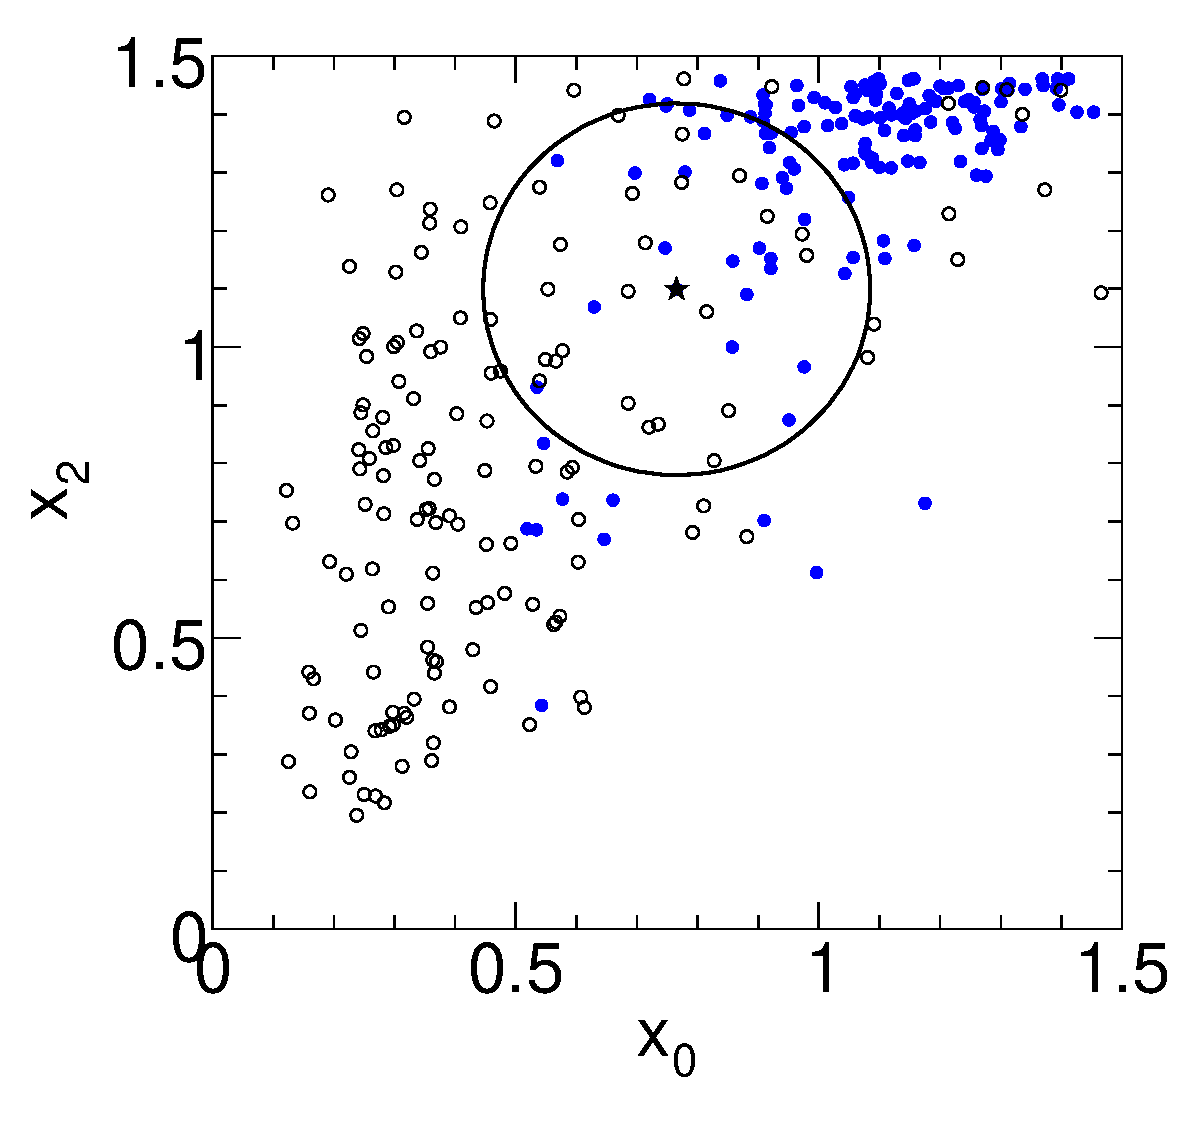
\includegraphics[width=0.6\textwidth]{backgrounds_chapter/figures/knn_3d_s13_b7_x02.pdf}
  \caption[$k-$Nearest Neighbor classifier example]{Example of the operation of
  a \kNN classifier.  The closest $k=50$ neighbors (those inside the circle) to a
  test point (indicated by the star marker) are selected. The probability that
  the star marker is a signal event is given the number of signal neighbors (blue
  markers) in the circle divided by $k$. Image credit:~\cite{TMVA}}
  \label{fig:KNN}
\end{figure}

The classification feature of a \kNN can be trivially adapted to parameterize a
fake--rate such that it is defined everywhere.  Examining the form of
Equation~\ref{eq:KNNEquation}, it is clear that by replacing $n_{sig}$ with
$n_{passed}$ and $n_{bkg}$ with $n_{failed}$, the equation is equivalent to the
tau--fake rate.  We thus ``train'' the \kNN with tau--candidates which pass the
tau identification as signal events and those which fail as background events.
The resulting classifier is a function which returns the expected fake--rate for
any point in the space of the parameterization.  The choice of $k$ must be
optimized.  When $k$ is low, the small number of neighbors causes large counting
fluctuations in the fake rate.  If $k$ is too large, the \kNN effectively
averages over a large area of the space of the variables\footnote{In the limit
$k\to\inf$, the \kNN output reduces to a single number.  In this extreme case,
all information about the dependence of the fake--rate on the variables is
lost.}.  For the training statistics available in the 2010 data, $k=20$ is found
to be the optimal choice.

\subsection{Results of Background Estimation}
%
An independent estimate of the background contributions to the analysis
presented in this thesis is obtained by applying the fake--rate method in a
manner analogous to the closure test.  Fake--rates in QCD multi--jet events
(light quark enriched sample), QCD events containing muons (heavy quark and
gluon enriched sample) and \WpJets events are measured in
data~\cite{CMS-PAS-PFT-10-004,CMS-PAS-TAU-11-001} and applied to events which
pass all the event selection criteria listed in
table~\ref{tab:AHtoMuTauEventSelection}, with the exceptions of 
\begin{itemize}
  \item the ``medium'' \hpsTanc discriminator, and
  \item the requirement that the tau have unit charge.
\end{itemize}

No assumption is made on the composition of \ZMM, \WpJets,
\ttbarpJets and QCD backgrounds contributing to the event sample selected
by the analysis.  Differences between fake--rates obtained for QCD multi--jet,
QCD muon enriched and \WpJets background events are attributed as systematic
uncertainties of the fake--rate method.  Per jet and per event weights have been
computed by the ``simple'' and ``CDF-type'' weights as described
in the closure test and the results are found to be compatible within
statistical and systematic uncertainties.  In the following, we present results
for ``CDF-type'' weights.  The ``CDF-type'' weights have the advantage that the
background estimate obtained does not change, whether there is MSSM Higgs $\to
\tau^{+} \tau^{-}$ signal present in the data or not.

Tau identification efficiencies need to be known when using ``CDF-type''
weights.  Dedicated studies have checked the tau identification efficiencies in
data~\cite{CMS-PAS-TAU-11-001}.  Statistical and systematic uncertainties of
these studies are still sizeable at present, in the order to $20-30\%$.  No
indication has been found, however, that the Monte Carlo simulation does not
correctly model hadronic tau decays in data.  For the purpose of computing
fake--rate weights via the ``CDF-type'' method, tau identification efficiencies
are taken from the Monte Carlo simulation of hadronic tau decays in \ZTT events.
Systematic uncertainties on the background estimate obtained by the fake--rate
method are determined by varying the tau identification efficiencies by $\pm
30\%$ relative to the value obtained from the Monte Carlo simulation.

The results of applying the fake--rate method to the mu + tau channel are
summarized in Table~\ref{tab:MuTauFakeRateResultsOS}.  The background prediction
has been corrected for the expected\footnote{The contribution of $\ZMM$ is
estimated using a simulated sample.} contribution of $13.1^{+2.8}_{-0.6}$ events
from $Z \to \mu^{+} \mu^{-}$ background events in which the reconstructed
tau--jet is due to a misidentified muon.  The obtained estimate is in good
agreement with the Monte Carlo expectation.
%
\begin{table}[t]
\begin{center}
\tablesize
\begin{tabular}{|l|c|c|}
\hline
Events weighted by: & Estimate \\
\hline
QCD lead jet       & $202.1^{+14.9}_{-74.8}$\\ % scaled 1.034 to account for tau code change
QCD second jet      & $198.0^{+22.8}_{-79.3}$\\% scaled 1.034 to account for tau code change
QCD $\mu$--enriched & $213.3^{+17.7}_{-82.6}$ \\
\WpJets          & $232.8^{+21.1}_{-95.0}$ \\
\hline
%$N_{bgr}$ estimate  & $223.0^{+23.9}_{-65.9}$ \\ - before Zmumu correction.
$N_{bgr}$ estimate  & $236.1^{+24.1}_{-65.9}$ \\ %- after Zmumu correction.
\hline
\end{tabular}
\end{center}
\begin{center}
\caption[Fake--rate method results]{Estimate for background contributions
obtained by weighting events passing all selection criteria listed in
Table~\ref{tab:AHtoMuTauEventSelection} except for the requirement for tau--jet
candidates to pass the ``medium'' tight TaNC discriminator and have unit charge
by fake--rates measured in QCD multi--jet, QCD muon enriched and \WpJets data
samples.} \label{tab:MuTauFakeRateResultsOS}
\end{center}
\end{table}

As an additional cross--check of the method, a sample of events containing a
muon plus a tau--jet of like--sign charge is selected in data and compared to
the background prediction obtained by applying the fake--rate method to the
like--sign sample.  The like--sign sample is expected to be dominated by the
contributions of \WpJets and QCD background processes and allows to verify the
fake--rate method in a practically signal free event sample.  The background
estimate obtained by the fake--rate method is compared to the number of events
observed in the like--sign data sample in
Table~\ref{tab:MuTauFakeRateResultsSS}.  The number of events expected in the
like--sign control sample from Monte Carlo simulation is indicated in the
caption.  All numbers are in good agreement.

The fake--rate method does not only allow to estimate the total number of
background events, but allows to model the distributions of background processes
as well.  The capability to model distributions is illustrated in
Figure~\ref{fig:MuTauFakeRateResultsSS}, which shows good agreement between the
distributions observed in the like-sign data sample and the predictions obtained
by the fake--rate method for the distributions of muon plus tau--jet visible
mass and of the ``full'' invariant mass reconstructed by the SVfit algorithm.
%
\begin{table}[t]
\begin{center}
\tablesize
\begin{tabular}{|l|c|c|}
\hline
Events weighted by:     & Estimate \\
\hline
QCD lead jet           & $191.7^{+2.3}_{-17.9}$ \\% scaled 1.034 to account for tau code change
QCD second jet          & $185.1^{+6.0}_{-21.1}$ \\% scaled 1.034 to account for tau code change
QCD $\mu$--enriched     & $194.7^{+2.0}_{-20.5}$ \\
\WpJets              & $208.9^{+0.5}_{-14.4}$ \\
\hline
Fake--rate estimate     & $201.8^{+14.2}_{-18.9}$ \\
\hline
Observed                & $216$ \\
\hline
\end{tabular}
\end{center}
\begin{center}
\caption[Fake--rate Method predicted yields in like--sign control region]{Number
of events observed in like--sign control region compared to estimate obtained by
fake--rate method.  } \label{tab:MuTauFakeRateResultsSS}
\end{center}
\end{table}
%
\begin{figure}[t]
\setlength{\unitlength}{1mm}
\begin{center}
\begin{picture}(150,52)(0,0)
\put(0.5, 2){\mbox{\includegraphics*[height=52mm, viewport=19 0 524 396]{backgrounds_chapter/figures/VisMass_SS_linear_bin_normed.pdf}}}
\put(78.0, 2){\mbox{\includegraphics*[height=52mm, viewport=19 0 524 396]{backgrounds_chapter/figures/SVfit_SS_linear_bin_normed.pdf}}}
\end{picture}
\caption[Comparison of visible mass and SVfit mass]{Distribution of visible mass
(left) and ``full'' invariant mass reconstructed by the SVfit algorithm (right)
observed in the like--sign charge control region compared to the background
estimate obtained by the fake--rate method.
} \label{fig:MuTauFakeRateResultsSS}
\end{center}
\end{figure} 
\fixme{THIS IS FROM THE HPS NOTE!}

\section{Template method}
\label{sec:template}
%
Shape templates for the $\mu + \tau_{had}$ visible mass $M_{vis}$ are obtained
from data, using a set of dedicated control regions which are chosen to select a
high purity sample of one particular background process each.  The number of
events selected in each control region and comparisons to the predictions from
Monte Carlo simulations are summarized in
Table~\ref{tab:ResultsMuTauBgControlRegions}.  The template $M_{vis}$ shapes
obtained from data in the background enriched control regions are compared to
the signal region shapes obtained by Monte Carlo simulation in
figure~\ref{fig:VisMassTemplates}.  The $M_{vis}$ spectrum observed in the final
analysis is fitted to the sum of these templates.  Estimates for background
yields are obtained from the normalization factor of each template, determined
by the fit.  Further details of the method can be found
in~\cite{CMS_AN_2010-088} and~\cite{CMS_AN_2011-021}. 
%
\begin{figure}
\setlength{\unitlength}{1mm}
\begin{center}
\begin{picture}(150,170)(0,0)
\put(0.5, 118){\mbox{\includegraphics*[width=52mm, angle=90]
  {backgrounds_chapter/figures/plotBgEstTemplateData_vs_AnalysisZtoMuTau_ZmumuMuonMisIdEnriched_visMass.pdf}}}
\put(78.0, 118){\mbox{\includegraphics*[width=52mm, angle=90]
  {backgrounds_chapter/figures/plotBgEstTemplateData_vs_AnalysisZtoMuTau_ZmumuJetMisIdEnriched_visMass.pdf}}}
\put(0.5, 60){\mbox{\includegraphics*[width=52mm, angle=90]
  {backgrounds_chapter/figures/plotBgEstTemplateData_vs_AnalysisZtoMuTau_WplusJetsEnriched_visMass.pdf}}}
\put(78.0, 60){\mbox{\includegraphics*[width=52mm, angle=90]
  {backgrounds_chapter/figures/plotBgEstTemplateData_vs_AnalysisZtoMuTau_WplusJetsEnriched_visMass_corrected.pdf}}}
\put(0.5, 2){\mbox{\includegraphics*[width=52mm, angle=90]
  {backgrounds_chapter/figures/plotBgEstTemplateData_vs_AnalysisZtoMuTau_TTplusJetsEnriched_visMass.pdf}}}
\put(78.0, 2){\mbox{\includegraphics*[width=52mm, angle=90]
  {backgrounds_chapter/figures/plotBgEstTemplateData_vs_AnalysisZtoMuTau_QCDenriched_visMass.pdf}}}
\put(-5.5, 170.5){\small (a)}
\put(72.0, 170.5){\small (b)}
\put(-5.5, 112.5){\small (c)}
\put(72.0, 112.5){\small (d)}
\put(-5.5, 54.5){\small (e)}
\put(72.0, 54.5){\small (f)}
\end{picture}
\caption[Comparison of background shapes in the signal and control
regions]{\captiontext $\mu + \tau_{had}$ shape templates obtained from $Z \to
\mu^{+} \mu^{-}$ (a) and (b), $W$ + jets before (c) and after (d) the bias
correction explained in Section~\ref{sec:template}, \ttbarpJets (e) and
QCD multi--jet (f) backgrounds enriched control regions compared to the expected
distribution of the of the enriched background process to the signal region,
predicted by Monte Carlo simulations.  In (a) reconstructed tau--jet candidates
are expected to be dominantly due to misidentified muons, while in (b) they are
expected to be mostly due to misidentified quark or gluon jets.}
\label{fig:VisMassTemplates}
\end{center}
\end{figure} 

The TaNC~(Section~\ref{sec:Tanc}, \cite{CMS_AN_2010-099}) discriminators used
in~\cite{CMS_AN_2011-021} are replaced by the corresponding discriminators of
the \hpsTanc algorithm~(Section~\ref{sec:TauId}, \cite{CMS_AN_2010-082}).  The
$Z/\gamma^{*} \to \tau^{+} \tau^{-}$ signal shape is obtained via the
$Z/\gamma^{*} \to \mu^{+} \mu^{-}$ embedding technique~\cite{MCEmbedding}.
\begin{figure}
\setlength{\unitlength}{1mm}
\begin{center}
\includegraphics*[width=62mm,
angle=90]{backgrounds_chapter/figures/fitBgEstTemplateZtoMuTau_visMass.pdf}
\caption[Visible mass distribution in the final fit of the Template
Method]{\captiontext $M_{vis}$ distribution of events selected by the
$Z/\gamma^{*} \rightarrow \tau^{+} \tau^{-} \rightarrow \mu + \tau_{had}$
cross--section analysis compared to the sum of shape templates for signal and
background processes scaled by the normalization factors determined by the fit.}
\label{fig:TemplateFitControlPlot}
\end{center}
\end{figure} 
The $\mu + \tau_{had}$ visible mass spectrum observed in the final analysis is
compared to the sum of template shapes scaled by the normalization factors
determined by the fit in Figure~\ref{fig:TemplateFitControlPlot}.  The
corresponding estimates for background contributions are summarized in
Table~\ref{tab:BgEstTemplateMethod}.
 %QCD: normalization = 130.547 +/- 35.1123 TTplusJets: normalization = 8.84426
 %+/- 6.7345 WplusJets: normalization = 80.2047 +/- 24.7961 ZmumuJetMisId:
 %normalization = 6.21001 +/- 5.72237 ZmumuMuonMisId: normalization =
 %8.77512e-05 +/- 7.37436 Ztautau: normalization = 296.405 +/- 30.7937

\begin{table}[t]
\begin{center}
\tablesize
\begin{tabular}{|l|c|c|c|c|c|c|c|c|}
\hline
Process & Estimate \\
\hline
\hline
\ZMM & \\
\hspace{2mm} Muon fake &    $5.7 \pm  6.0$ \\
\hspace{2mm} Jet fake  & $< 14.5$ \\
\WpJets
\ttbarpJets          &    $7.6 \pm  6.9$ \\
QCD                        &  $141.3 \pm 40.4$ \\
\hline
$N_{bgr}$ estimate         &  $226.5 \pm 33.1$ \\
\hline
\end{tabular}
\caption[Background yields measured using the Template Method]{\captiontext
Estimated contributions of individual background processes to the signal region,
obtained via the template method.  As the shapes are very similar, the
normalization factors for QCD and \WpJets background processes are
anti--correlated.  As a consequence, the sum of background contributions is
determined by the fit more precisely than the individual contributions.}
\label{tab:BgEstTemplateMethod}
\end{center}
\end{table}
\ifx\master\undefined% AUTOCOMPILE
% Allows for individual chapters to be compiled.

% Usage:
% \ifx\master\undefined% AUTOCOMPILE
% Allows for individual chapters to be compiled.

% Usage:
% \ifx\master\undefined% AUTOCOMPILE
% Allows for individual chapters to be compiled.

% Usage:
% \ifx\master\undefined\input{../settings/autocompile}\fi
% (place at start and end of chapter file)

\ifx\noprelim\undefined
    % first time included
    % input preamble files
    \input{../settings/phdsetup}

    \begin{document}
    \def\noprelim{}
\else
    % already included once
    % input post files

    \singlespacing
    \bibliographystyle{../bibliography/expanded}
    \bibliography{../bibliography/references}

    \end{document}
\fi\fi
% (place at start and end of chapter file)

\ifx\noprelim\undefined
    % first time included
    % input preamble files
    % [ USER VARIABLES ]

\def\PHDTITLE {Extensions of the Theory of Computational Mechanics}
\def\PHDAUTHOR{Evan Klose Friis}
\def\PHDSCHOOL{University of California, Davis}

\def\PHDMONTH {June}
\def\PHDYEAR  {2011}
\def\PHDDEPT {Physics}

\def\BSSCHOOL {University of California at San Diego}
\def\BSYEAR   {2005}

\def\PHDCOMMITTEEA{Professor John Conway}
\def\PHDCOMMITTEEB{Professor Robin Erbacher}
\def\PHDCOMMITTEEC{Professor Mani Tripathi}

% [ GLOBAL SETUP ]

\documentclass[letterpaper,oneside,11pt]{report}

\usepackage{calc}
\usepackage{breakcites}
\usepackage[newcommands]{ragged2e}

\usepackage[pdftex]{graphicx}
\usepackage{epstopdf}

%\usepackage{tikz}
%\usetikzlibrary{positioning} % [right=of ...]
%\usetikzlibrary{fit} % [fit= ...]

%\pgfdeclarelayer{background layer}
%\pgfdeclarelayer{foreground layer}
%\pgfsetlayers{background layer,main,foreground layer}

%\newenvironment{wrap}{\noindent\begin{minipage}[t]{\linewidth}\vspace{-0.5\normalbaselineskip}\centering}{\vspace{0.5\normalbaselineskip}\end{minipage}}

%% [Venn diagram environment]
%\newenvironment{venn2}
%{\begin{tikzpicture} [every pin/.style={text=black, text opacity=1.0, pin distance=0.5cm, pin edge={black!60, semithick}},
%% define a new style 'venn'
%venn/.style={circle, draw=black!60, semithick, minimum size = 4cm}]
%
%% create circle and give it external (pin) label
%\node[venn] (X) at (-1,0) [pin={150:$H[X]$}] {};
%\node[venn] (Y) at (1,0) [pin={30:$H[Y]$}] {};
%
%% place labels of the atoms by hand
%\node at (-1.9,0) {$H[X|Y]$};
%\node at (1.9,0) {$H[Y|X]$};
%\node at (0,0) {$I[X;Y]$};}
%{\end{tikzpicture}}

%\newcommand{\wrapmath}[1]{\begin{wrap}\begin{tikzpicture}[every node/.style={inner ysep=0ex, inner xsep=0em}]\node[] {$\displaystyle\begin{aligned} #1\end{aligned}$};\end{tikzpicture}\end{wrap}}

\renewenvironment{abstract}{\chapter*{Abstract}}{}
\renewcommand{\bibname}{Bibliography}
\renewcommand{\contentsname}{Table of Contents}

\makeatletter
\renewcommand{\@biblabel}[1]{\textsc{#1}}
\makeatother

% [ FONT SETTINGS ]

\usepackage[tbtags, intlimits, namelimits]{amsmath}
\usepackage[adobe-utopia]{mathdesign}

\DeclareSymbolFont{pazomath}{OMS}{zplm}{m}{n}
\DeclareSymbolFontAlphabet{\mathcal}{pazomath}
\SetMathAlphabet\mathcal{bold}{OMS}{zplm}{b}{n}

\SetSymbolFont{largesymbols}{normal}{OMX}{zplm}{m}{n}
\SetSymbolFont{largesymbols}{bold}{OMX}{zplm}{m}{n}
\SetSymbolFont{symbols}{normal}{OMS}{zplm}{m}{n}
\SetSymbolFont{symbols}{bold}{OMS}{zplm}{b}{n}

\renewcommand{\sfdefault}{phv}
\renewcommand{\ttdefault}{fvm}

\widowpenalty 8000
\clubpenalty  8000

% [ PAGE LAYOUT ]
\usepackage{geometry}
\geometry{lmargin = 1.5in}
\geometry{rmargin = 1.0in}
\geometry{tmargin = 1.0in}
\geometry{bmargin = 1.0in}

% [ PDF SETTINGS ]

\usepackage[final]{hyperref}
\hypersetup{breaklinks  = true}
\hypersetup{colorlinks  = true}
\hypersetup{linktocpage = false}
\hypersetup{linkcolor   = blue}
\hypersetup{citecolor   = green}
\hypersetup{urlcolor    = black}
\hypersetup{plainpages  = false}
\hypersetup{pageanchor  = true}
\hypersetup{pdfauthor   = {\PHDAUTHOR}}
\hypersetup{pdftitle    = {\PHDTITLE}}
\hypersetup{pdfsubject  = {Dissertation, \PHDSCHOOL}}
\urlstyle{same}

% [ LETTER SPACING ]

\usepackage[final]{microtype}
\microtypesetup{protrusion=compatibility}
\microtypesetup{expansion=false}

\newcommand{\upper}[1]{\MakeUppercase{#1}}
\let\lsscshape\scshape

\ifcase\pdfoutput\else\microtypesetup{letterspace=15}
\renewcommand{\scshape}{\lsscshape\lsstyle}
\renewcommand{\upper}[1]{\textls[50]{\MakeUppercase{#1}}}\fi

% [ LINE SPACING ]

\usepackage[doublespacing]{setspace}
\renewcommand{\displayskipstretch}{0.0}

\setlength{\parskip   }{0em}
\setlength{\parindent }{2em}

% [ TABLE FORMATTING ]

\usepackage{booktabs}
\setlength{\heavyrulewidth}{1.5\arrayrulewidth}
\setlength{\lightrulewidth}{1.0\arrayrulewidth}
\setlength{\doublerulesep }{2.0\arrayrulewidth}

% [ SECTION FORMATTING ]

\usepackage[largestsep,nobottomtitles*]{titlesec}
\renewcommand{\bottomtitlespace}{0.75in}

\titleformat{\chapter}[display]{\bfseries\huge\singlespacing}{\filleft\textsc{\LARGE \chaptertitlename\ \thechapter}}{-0.2ex}{\titlerule[3pt]\vspace{0.2ex}}[]

\titleformat{\section}{\LARGE}{\S\thesection\hspace{0.5em}}{0ex}{}
\titleformat{\subsection}{\Large}{\S\thesubsection\hspace{0.5em}}{0ex}{}
\titleformat{\subsubsection}{\large}{\thesubsubsection\hspace{0.5em}}{0ex}{}

\titlespacing*{\chapter}{0em}{6ex}{4ex plus 2ex minus 0ex}
\titlespacing*{\section}{0em}{2ex plus 3ex minus 1ex}{0.5ex plus 0.5ex minus 0.5ex}
\titlespacing*{\subsection}{0ex}{2ex plus 3ex minus 1ex}{0ex}
\titlespacing*{\subsubsection}{0ex}{2ex plus 0ex minus 1ex}{0ex}

% [ HEADER SETTINGS ]

\usepackage{fancyhdr}

\setlength{\headheight}{\normalbaselineskip}
\setlength{\footskip  }{0.5in}
\setlength{\headsep   }{0.5in-\headheight}

\fancyheadoffset[R]{0.5in}
\renewcommand{\headrulewidth}{0pt}
\renewcommand{\footrulewidth}{0pt}

\newcommand{\pagebox}{\parbox[r][\headheight][t]{0.5in}{\hspace\fill\thepage}}

\newcommand{\prelimheaders}{\ifx\prelim\undefined\renewcommand{\thepage}{\textit{\roman{page}}}\fancypagestyle{plain}{\fancyhf{}\fancyfoot[L]{\makebox[\textwidth-0.5in]{\thepage}}}\pagestyle{plain}\def\prelim{}\fi}

\newcommand{\normalheaders}{\renewcommand{\thepage}{\arabic{page}}\fancypagestyle{plain}{\fancyhf{}\fancyhead[R]{\pagebox}}\pagestyle{plain}}

\normalheaders{}

% [ CUSTOM COMMANDS ]

\newcommand{\signaturebox}[1]{\multicolumn{1}{p{4in}}{\vspace{3ex}}\\\midrule #1\\}

%\input{../includes/cmechabbrev}

% [some math stuff - maybe stick in sep file]
\usepackage{amsthm}
\usepackage{amscd}
\theoremstyle{plain}    \newtheorem{Lem}{Lemma}
\theoremstyle{plain}    \newtheorem*{ProLem}{Proof}
\theoremstyle{plain} 	\newtheorem{Cor}{Corollary}
\theoremstyle{plain} 	\newtheorem*{ProCor}{Proof}
\theoremstyle{plain} 	\newtheorem{The}{Theorem}
\theoremstyle{plain} 	\newtheorem*{ProThe}{Proof}
\theoremstyle{plain} 	\newtheorem{Prop}{Proposition}
\theoremstyle{plain} 	\newtheorem*{ProProp}{Proof}
\theoremstyle{plain} 	\newtheorem*{Conj}{Conjecture}
\theoremstyle{plain}	\newtheorem*{Rem}{Remark}
\theoremstyle{plain}	\newtheorem*{Def}{Definition} 
\theoremstyle{plain}	\newtheorem*{Not}{Notation}

% [uniform figure scaling - maybe this is not a good idea]
\def\figscale{.7}
\def\lscale{1.0}

% [FIX ME! - red makes it easier to spot]
\newcommand{\FIX}[1]{\textbf{\textcolor{red}{#1}}}


    \begin{document}
    \def\noprelim{}
\else
    % already included once
    % input post files

    \singlespacing
    \bibliographystyle{../bibliography/expanded}
    \bibliography{../bibliography/references}

    \end{document}
\fi\fi
% (place at start and end of chapter file)

\ifx\noprelim\undefined
    % first time included
    % input preamble files
    % [ USER VARIABLES ]

\def\PHDTITLE {Extensions of the Theory of Computational Mechanics}
\def\PHDAUTHOR{Evan Klose Friis}
\def\PHDSCHOOL{University of California, Davis}

\def\PHDMONTH {June}
\def\PHDYEAR  {2011}
\def\PHDDEPT {Physics}

\def\BSSCHOOL {University of California at San Diego}
\def\BSYEAR   {2005}

\def\PHDCOMMITTEEA{Professor John Conway}
\def\PHDCOMMITTEEB{Professor Robin Erbacher}
\def\PHDCOMMITTEEC{Professor Mani Tripathi}

% [ GLOBAL SETUP ]

\documentclass[letterpaper,oneside,11pt]{report}

\usepackage{calc}
\usepackage{breakcites}
\usepackage[newcommands]{ragged2e}

\usepackage[pdftex]{graphicx}
\usepackage{epstopdf}

%\usepackage{tikz}
%\usetikzlibrary{positioning} % [right=of ...]
%\usetikzlibrary{fit} % [fit= ...]

%\pgfdeclarelayer{background layer}
%\pgfdeclarelayer{foreground layer}
%\pgfsetlayers{background layer,main,foreground layer}

%\newenvironment{wrap}{\noindent\begin{minipage}[t]{\linewidth}\vspace{-0.5\normalbaselineskip}\centering}{\vspace{0.5\normalbaselineskip}\end{minipage}}

%% [Venn diagram environment]
%\newenvironment{venn2}
%{\begin{tikzpicture} [every pin/.style={text=black, text opacity=1.0, pin distance=0.5cm, pin edge={black!60, semithick}},
%% define a new style 'venn'
%venn/.style={circle, draw=black!60, semithick, minimum size = 4cm}]
%
%% create circle and give it external (pin) label
%\node[venn] (X) at (-1,0) [pin={150:$H[X]$}] {};
%\node[venn] (Y) at (1,0) [pin={30:$H[Y]$}] {};
%
%% place labels of the atoms by hand
%\node at (-1.9,0) {$H[X|Y]$};
%\node at (1.9,0) {$H[Y|X]$};
%\node at (0,0) {$I[X;Y]$};}
%{\end{tikzpicture}}

%\newcommand{\wrapmath}[1]{\begin{wrap}\begin{tikzpicture}[every node/.style={inner ysep=0ex, inner xsep=0em}]\node[] {$\displaystyle\begin{aligned} #1\end{aligned}$};\end{tikzpicture}\end{wrap}}

\renewenvironment{abstract}{\chapter*{Abstract}}{}
\renewcommand{\bibname}{Bibliography}
\renewcommand{\contentsname}{Table of Contents}

\makeatletter
\renewcommand{\@biblabel}[1]{\textsc{#1}}
\makeatother

% [ FONT SETTINGS ]

\usepackage[tbtags, intlimits, namelimits]{amsmath}
\usepackage[adobe-utopia]{mathdesign}

\DeclareSymbolFont{pazomath}{OMS}{zplm}{m}{n}
\DeclareSymbolFontAlphabet{\mathcal}{pazomath}
\SetMathAlphabet\mathcal{bold}{OMS}{zplm}{b}{n}

\SetSymbolFont{largesymbols}{normal}{OMX}{zplm}{m}{n}
\SetSymbolFont{largesymbols}{bold}{OMX}{zplm}{m}{n}
\SetSymbolFont{symbols}{normal}{OMS}{zplm}{m}{n}
\SetSymbolFont{symbols}{bold}{OMS}{zplm}{b}{n}

\renewcommand{\sfdefault}{phv}
\renewcommand{\ttdefault}{fvm}

\widowpenalty 8000
\clubpenalty  8000

% [ PAGE LAYOUT ]
\usepackage{geometry}
\geometry{lmargin = 1.5in}
\geometry{rmargin = 1.0in}
\geometry{tmargin = 1.0in}
\geometry{bmargin = 1.0in}

% [ PDF SETTINGS ]

\usepackage[final]{hyperref}
\hypersetup{breaklinks  = true}
\hypersetup{colorlinks  = true}
\hypersetup{linktocpage = false}
\hypersetup{linkcolor   = blue}
\hypersetup{citecolor   = green}
\hypersetup{urlcolor    = black}
\hypersetup{plainpages  = false}
\hypersetup{pageanchor  = true}
\hypersetup{pdfauthor   = {\PHDAUTHOR}}
\hypersetup{pdftitle    = {\PHDTITLE}}
\hypersetup{pdfsubject  = {Dissertation, \PHDSCHOOL}}
\urlstyle{same}

% [ LETTER SPACING ]

\usepackage[final]{microtype}
\microtypesetup{protrusion=compatibility}
\microtypesetup{expansion=false}

\newcommand{\upper}[1]{\MakeUppercase{#1}}
\let\lsscshape\scshape

\ifcase\pdfoutput\else\microtypesetup{letterspace=15}
\renewcommand{\scshape}{\lsscshape\lsstyle}
\renewcommand{\upper}[1]{\textls[50]{\MakeUppercase{#1}}}\fi

% [ LINE SPACING ]

\usepackage[doublespacing]{setspace}
\renewcommand{\displayskipstretch}{0.0}

\setlength{\parskip   }{0em}
\setlength{\parindent }{2em}

% [ TABLE FORMATTING ]

\usepackage{booktabs}
\setlength{\heavyrulewidth}{1.5\arrayrulewidth}
\setlength{\lightrulewidth}{1.0\arrayrulewidth}
\setlength{\doublerulesep }{2.0\arrayrulewidth}

% [ SECTION FORMATTING ]

\usepackage[largestsep,nobottomtitles*]{titlesec}
\renewcommand{\bottomtitlespace}{0.75in}

\titleformat{\chapter}[display]{\bfseries\huge\singlespacing}{\filleft\textsc{\LARGE \chaptertitlename\ \thechapter}}{-0.2ex}{\titlerule[3pt]\vspace{0.2ex}}[]

\titleformat{\section}{\LARGE}{\S\thesection\hspace{0.5em}}{0ex}{}
\titleformat{\subsection}{\Large}{\S\thesubsection\hspace{0.5em}}{0ex}{}
\titleformat{\subsubsection}{\large}{\thesubsubsection\hspace{0.5em}}{0ex}{}

\titlespacing*{\chapter}{0em}{6ex}{4ex plus 2ex minus 0ex}
\titlespacing*{\section}{0em}{2ex plus 3ex minus 1ex}{0.5ex plus 0.5ex minus 0.5ex}
\titlespacing*{\subsection}{0ex}{2ex plus 3ex minus 1ex}{0ex}
\titlespacing*{\subsubsection}{0ex}{2ex plus 0ex minus 1ex}{0ex}

% [ HEADER SETTINGS ]

\usepackage{fancyhdr}

\setlength{\headheight}{\normalbaselineskip}
\setlength{\footskip  }{0.5in}
\setlength{\headsep   }{0.5in-\headheight}

\fancyheadoffset[R]{0.5in}
\renewcommand{\headrulewidth}{0pt}
\renewcommand{\footrulewidth}{0pt}

\newcommand{\pagebox}{\parbox[r][\headheight][t]{0.5in}{\hspace\fill\thepage}}

\newcommand{\prelimheaders}{\ifx\prelim\undefined\renewcommand{\thepage}{\textit{\roman{page}}}\fancypagestyle{plain}{\fancyhf{}\fancyfoot[L]{\makebox[\textwidth-0.5in]{\thepage}}}\pagestyle{plain}\def\prelim{}\fi}

\newcommand{\normalheaders}{\renewcommand{\thepage}{\arabic{page}}\fancypagestyle{plain}{\fancyhf{}\fancyhead[R]{\pagebox}}\pagestyle{plain}}

\normalheaders{}

% [ CUSTOM COMMANDS ]

\newcommand{\signaturebox}[1]{\multicolumn{1}{p{4in}}{\vspace{3ex}}\\\midrule #1\\}

%%%% macros fro standard references
%\eqref provided by amsmath
\newcommand{\figref}[1]{Fig.~\ref{#1}}
\newcommand{\tableref}[1]{Table~\ref{#1}}
\newcommand{\refcite}[1]{Ref.~\cite{#1}}

% Abbreviations from CMPPSS:

\newcommand{\eM}     {\mbox{$\epsilon$-machine}}
\newcommand{\eMs}    {\mbox{$\epsilon$-machines}}
\newcommand{\EM}     {\mbox{$\epsilon$-Machine}}
\newcommand{\EMs}    {\mbox{$\epsilon$-Machines}}
\newcommand{\eT}     {\mbox{$\epsilon$-transducer}}
\newcommand{\eTs}    {\mbox{$\epsilon$-transducers}}
\newcommand{\ET}     {\mbox{$\epsilon$-Transducer}}
\newcommand{\ETs}    {\mbox{$\epsilon$-Transducers}}

% Processes and sequences

\newcommand{\Process}{\mathcal{P}}

\newcommand{\ProbMach}{\Prob_{\mathrm{M}}}
\newcommand{\Lmax}   { {L_{\mathrm{max}}}}
\newcommand{\MeasAlphabet}	{\mathcal{A}}
% Original
%\newcommand{\MeasSymbol}   { {S} }
%\newcommand{\meassymbol}   { {s} }
% New symbol
\newcommand{\MeasSymbol}   { {X} }
\newcommand{\meassymbol}   { {x} }
\newcommand{\BiInfinity}	{ \overleftrightarrow {\MeasSymbol} }
\newcommand{\biinfinity}	{ \overleftrightarrow {\meassymbol} }
\newcommand{\Past}	{ \overleftarrow {\MeasSymbol} }
\newcommand{\past}	{ {\overleftarrow {\meassymbol}} }
\newcommand{\pastprime}	{ {\past}^{\prime}}
\newcommand{\Future}	{ \overrightarrow{\MeasSymbol} }
\newcommand{\future}	{ \overrightarrow{\meassymbol} }
\newcommand{\futureprime}	{ {\future}^{\prime}}
\newcommand{\PastPrime}	{ {\Past}^{\prime}}
\newcommand{\FuturePrime}	{ {\overrightarrow{\meassymbol}}^\prime }
\newcommand{\PastDblPrime}	{ {\overleftarrow{\meassymbol}}^{\prime\prime} }
\newcommand{\FutureDblPrime}	{ {\overrightarrow{\meassymbol}}^{\prime\prime} }
\newcommand{\pastL}	{ {\overleftarrow {\meassymbol}}{}^L }
\newcommand{\PastL}	{ {\overleftarrow {\MeasSymbol}}{}^L }
\newcommand{\PastLt}	{ {\overleftarrow {\MeasSymbol}}_t^L }
\newcommand{\PastLLessOne}	{ {\overleftarrow {\MeasSymbol}}^{L-1} }
\newcommand{\futureL}	{ {\overrightarrow{\meassymbol}}{}^L }
\newcommand{\FutureL}	{ {\overrightarrow{\MeasSymbol}}{}^L }
\newcommand{\FutureLt}	{ {\overrightarrow{\MeasSymbol}}_t^L }
\newcommand{\FutureLLessOne}	{ {\overrightarrow{\MeasSymbol}}^{L-1} }
\newcommand{\pastLprime}	{ {\overleftarrow {\meassymbol}}^{L^\prime} }
\newcommand{\futureLprime}	{ {\overrightarrow{\meassymbol}}^{L^\prime} }
\newcommand{\AllPasts}	{ { \overleftarrow {\rm {\bf \MeasSymbol}} } }
\newcommand{\AllFutures}	{ \overrightarrow {\rm {\bf \MeasSymbol}} }
\newcommand{\FutureSet}	{ \overrightarrow{\bf \MeasSymbol}}

% Causal states and epsilon-machines
\newcommand{\CausalState}	{ \mathcal{S} }
\newcommand{\CausalStatePrime}	{ {\CausalState}^{\prime}}
\newcommand{\causalstate}	{ \sigma }
\newcommand{\CausalStateSet}	{ \boldsymbol{\CausalState} }
\newcommand{\AlternateState}	{ \mathcal{R} }
\newcommand{\AlternateStatePrime}	{ {\cal R}^{\prime} }
\newcommand{\alternatestate}	{ \rho }
\newcommand{\alternatestateprime}	{ {\rho^{\prime}} }
\newcommand{\AlternateStateSet}	{ \boldsymbol{\AlternateState} }
\newcommand{\PrescientState}	{ \widehat{\AlternateState} }
\newcommand{\prescientstate}	{ \widehat{\alternatestate} }
\newcommand{\PrescientStateSet}	{ \boldsymbol{\PrescientState}}
\newcommand{\CausalEquivalence}	{ {\sim}_{\epsilon} }
\newcommand{\CausalEquivalenceNot}	{ {\not \sim}_{\epsilon}}

\newcommand{\NonCausalEquivalence}	{ {\sim}_{\eta} }
\newcommand{\NextObservable}	{ {\overrightarrow {\MeasSymbol}}^1 }
\newcommand{\LastObservable}	{ {\overleftarrow {\MeasSymbol}}^1 }
%\newcommand{\Prob}		{ {\rm P}}
\newcommand{\Prob}      {\Pr} % use standard command
\newcommand{\ProbAnd}	{ {,\;} }
\newcommand{\LLimit}	{ {L \rightarrow \infty}}
\newcommand{\Cmu}		{C_\mu}
\newcommand{\hmu}		{h_\mu}
\newcommand{\EE}		{{\bf E}}
\newcommand{\Measurable}{{\bf \mu}}

% Process Crypticity
\newcommand{\PC}		{\chi}
\newcommand{\FuturePC}		{\PC^+}
\newcommand{\PastPC}		{\PC^-}
% Causal Irreversibility
\newcommand{\CI}		{\Xi}
\newcommand{\ReverseMap}	{r}
\newcommand{\ForwardMap}	{f}

% Abbreviations from IB:
% None that aren't already in CMPPSS

% Abbreviations from Extensive Estimation:
\newcommand{\EstCausalState}	{\widehat{\CausalState}}
\newcommand{\estcausalstate}	{\widehat{\causalstate}}
\newcommand{\EstCausalStateSet}	{\boldsymbol{\EstCausalState}}
\newcommand{\EstCausalFunc}	{\widehat{\epsilon}}
\newcommand{\EstCmu}		{\widehat{\Cmu}}
\newcommand{\PastLOne}	{{\Past}^{L+1}}
\newcommand{\pastLOne}	{{\past}^{L+1}}

% Abbreviations from $\epsilon$-Transducers:
\newcommand{\InAlphabet}	{ \mathcal{A}}
\newcommand{\insymbol}		{ a}
\newcommand{\OutAlphabet}	{ \mathcal{B}}
\newcommand{\outsymbol}		{ b}
\newcommand{\InputSimple}	{ X}
\newcommand{\inputsimple}	{ x}
\newcommand{\BottleneckVar}	{\tilde{\InputSimple}}
\newcommand{\bottleneckvar}	{\tilde{\inputsimple}}
\newcommand{\InputSpace}	{ \mathbf{\InputSimple}}
\newcommand{\InputBi}	{ \overleftrightarrow {\InputSimple} }
\newcommand{\inputbi}	{ \overleftrightarrow {\inputsimple} }
\newcommand{\InputPast}	{ \overleftarrow {\InputSimple} }
\newcommand{\inputpast}	{ \overleftarrow {\inputsimple} }
\newcommand{\InputFuture}	{ \overrightarrow {\InputSimple} }
\newcommand{\inputfuture}	{ \overrightarrow {\inputsimple} }
\newcommand{\NextInput}	{ {{\InputFuture}^{1}}}
\newcommand{\NextOutput}	{ {\OutputFuture}^{1}}
\newcommand{\OutputSimple}	{ Y}
\newcommand{\outputsimple}	{ y}
\newcommand{\OutputSpace}	{ \mathbf{\OutputSimple}}
\newcommand{\OutputBi}	{ \overleftrightarrow{\OutputSimple} }
\newcommand{\outputbi}	{ \overleftrightarrow{\outputsimple} }
\newcommand{\OutputPast}	{ \overleftarrow{\OutputSimple} }
\newcommand{\outputpast}	{ \overleftarrow{\outputsimple} }
\newcommand{\OutputFuture}	{ \overrightarrow{\OutputSimple} }
\newcommand{\outputfuture}	{ \overrightarrow{\outputsimple} }
\newcommand{\OutputL}	{ {\OutputFuture}^L}
\newcommand{\outputL}	{ {\outputfuture}^L}
\newcommand{\InputLLessOne}	{ {\InputFuture}^{L-1}}
\newcommand{\inputLlessone}	{ {\inputufutre}^{L-1}}
\newcommand{\OutputPastLLessOne}	{{\OutputPast}^{L-1}_{-1}}
\newcommand{\outputpastLlessone}	{{\outputpast}^{L-1}}
\newcommand{\OutputPastLessOne}	{{\OutputPast}_{-1}}
\newcommand{\outputpastlessone}	{{\outputpast}_{-1}}
\newcommand{\OutputPastL}	{{\OutputPast}^{L}}
\newcommand{\OutputLPlusOne}	{ {\OutputFuture}^{L+1}}
\newcommand{\outputLplusone}	{ {\outputfutre}^{L+1}}
\newcommand{\InputPastL}	{{\InputPast}^{L}}
\newcommand{\inputpastL}	{{\inputpast}^{L}}
\newcommand{\JointPast}	{{(\InputPast,\OutputPast)}}
\newcommand{\jointpast}	{{(\inputpast,\outputpast)}}
\newcommand{\jointpastone}	{{(\inputpast_1,\outputpast_1)}}
\newcommand{\jointpasttwo}	{{(\inputpast_2,\outputpast_2)}}
\newcommand{\jointpastprime} {{({\inputpast}^{\prime},{\outputpast}^{\prime})}}
\newcommand{\NextJoint}	{{(\NextInput,\NextOutput)}}
\newcommand{\nextjoint}	{{(\insymbol,\outsymbol)}}
\newcommand{\AllInputPasts}	{ { \overleftarrow {\rm \InputSpace}}}
\newcommand{\AllOutputPasts}	{ {\overleftarrow {\rm \OutputSpace}}}
\newcommand{\DetCausalState}	{ {{\cal S}_D }}
\newcommand{\detcausalstate}	{ {{\sigma}_D} }
\newcommand{\DetCausalStateSet}	{ \boldsymbol{{\CausalState}_D}}
\newcommand{\DetCausalEquivalence}	{ {\sim}_{{\epsilon}_{D}}}
\newcommand{\PrescientEquivalence}	{ {\sim}_{\widehat{\eta}}}
\newcommand{\FeedbackCausalState}	{ \mathcal{F}}
\newcommand{\feedbackcausalstate}	{ \phi}
\newcommand{\FeedbackCausalStateSet}	{ \mathbf{\FeedbackCausalState}}
\newcommand{\JointCausalState}		{ \mathcal{J}}
\newcommand{\JointCausalStateSet}	{ \mathbf{\JointCausalState}}
\newcommand{\UtilityFunctional}	{ {\mathcal{L}}}
\newcommand{\NatureState}	{ {\Omega}}
\newcommand{\naturestate}	{ {\omega}}
\newcommand{\NatureStateSpace}	{ {\mathbf{\NatureState}}}
\newcommand{\AnAction}	{ {A}}
\newcommand{\anaction}	{ {a}}
\newcommand{\ActionSpace}	{ {\mathbf{\AnAction}}}

% Abbreviations from RURO:
\newcommand{\InfoGain}[2] { \mathcal{D} \left( {#1} || {#2} \right) }

% Abbreviations from Upper Bound:
\newcommand{\lcm}	{{\rm lcm}}
% Double-check that this isn't in the math set already!

% Abbreviations from Emergence in Space
\newcommand{\ProcessAlphabet}	{\MeasAlphabet}
\newcommand{\ProbEst}			{ {\widehat{\Prob}_N}}
\newcommand{\STRegion}			{ {\mathrm K}}
\newcommand{\STRegionVariable}		{ K}
\newcommand{\stregionvariable}		{ k}
\newcommand{\GlobalPast}		{ \overleftarrow{G}} 
\newcommand{\globalpast}		{ \overleftarrow{g}} 
\newcommand{\GlobalFuture}		{ \overrightarrow{G}}
\newcommand{\globalfuture}		{ \overrightarrow{g}}
\newcommand{\GlobalState}		{ \mathcal{G}}
\newcommand{\globalstate}		{ \gamma}
\newcommand{\GlobalStateSet}		{ {\mathbf \GlobalState}}
\newcommand{\LocalPast}			{ \overleftarrow{L}} 
\newcommand{\localpast}			{ \overleftarrow{l}}
\newcommand{\AllLocalPasts}		{ \mathbf{\LocalPast}}
\newcommand{\LocalPastRegion}		{ \overleftarrow{\mathrm L}}
\newcommand{\LocalFuture}		{ \overrightarrow{L}}
\newcommand{\localfuture}		{ \overrightarrow{l}}
\newcommand{\LocalFutureRegion}		{ \overrightarrow{\mathrm L}}
\newcommand{\LocalState}		{ \mathcal{L}}
\newcommand{\localstate}		{ \lambda}
\newcommand{\LocalStateSet}		{ {\mathbf \LocalState}}
\newcommand{\PatchPast}			{ \overleftarrow{P}}
\newcommand{\patchpast}			{ \overleftarrow{p}}
\newcommand{\PatchPastRegion}		{ \overleftarrow{\mathrm P}}
\newcommand{\PatchFuture}		{ \overrightarrow{P}}
\newcommand{\patchfuture}		{ \overrightarrow{p}}
\newcommand{\PatchFutureRegion}		{ \overrightarrow{\mathrm P}}
\newcommand{\PatchState}		{ \mathcal{P}}
\newcommand{\patchstate}		{ \pi}
\newcommand{\PatchStateSet}		{ {\mathbf \PatchState}}
\newcommand{\LocalStatesInPatch}	{\vec{\LocalState}}
\newcommand{\localstatesinpatch}	{\vec{\localstate}}
\newcommand{\PointInstantX}		{ {\mathbf x}}
% Galles's original LaTeX for the cond. indep. symbol follows:
\newcommand{\compos}{\mbox{$~\underline{~\parallel~}~$}}
\newcommand{\ncompos}{\not\hspace{-.15in}\compos}
\newcommand{\indep}			{ \rotatebox{90}{$\models$}}
\newcommand{\nindep}	{\not\hspace{-.05in}\indep}
\newcommand{\LocalEE}	{{\EE}^{loc}}
\newcommand{\EEDensity}	{\overline{\LocalEE}}
\newcommand{\LocalCmu}	{{\Cmu}^{loc}}
\newcommand{\CmuDensity}	{\overline{\LocalCmu}}

%%%%%%%%%%% added by sasa
\newcommand{\FinPast}[1]	{ \overleftarrow {\MeasSymbol} \stackrel{{#1}}{}}
\newcommand{\finpast}[1]  	{ \overleftarrow {\meassymbol}  \stackrel{{#1}}{}}
\newcommand{\FinFuture}[1]		{ \overrightarrow{\MeasSymbol} \stackrel{{#1}}{}}
\newcommand{\finfuture}[1]		{ \overrightarrow{\meassymbol} \stackrel{{#1}}{}}

\newcommand{\Partition}	{ \AlternateState }
\newcommand{\partitionstate}	{ \alternatestate }
\newcommand{\PartitionSet}	{ \AlternateStateSet }
\newcommand{\Fdet}   { F_{\rm det} }

\newcommand{\Dkl}[2] { D_{\rm KL} \left( {#1} || {#2} \right) }

\newcommand{\Period}	{p}

% To take into account time direction
\newcommand{\forward}{+}
\newcommand{\reverse}{-}
%\newcommand{\forwardreverse}{\:\!\diamond} % \pm
\newcommand{\forwardreverse}{\pm} % \pm
\newcommand{\FutureProcess}	{ {\Process}^{\forward} }
\newcommand{\PastProcess}	{ {\Process}^{\reverse} }
\newcommand{\FutureCausalState}	{ {\CausalState}^{\forward} }
\newcommand{\futurecausalstate}	{ \sigma^{\forward} }
\newcommand{\altfuturecausalstate}	{ \sigma^{\forward\prime} }
\newcommand{\PastCausalState}	{ {\CausalState}^{\reverse} }
\newcommand{\pastcausalstate}	{ \sigma^{\reverse} }
\newcommand{\BiCausalState}		{ {\CausalState}^{\forwardreverse} }
\newcommand{\bicausalstate}		{ {\sigma}^{\forwardreverse} }
\newcommand{\FutureCausalStateSet}	{ {\CausalStateSet}^{\forward} }
\newcommand{\PastCausalStateSet}	{ {\CausalStateSet}^{\reverse} }
\newcommand{\BiCausalStateSet}	{ {\CausalStateSet}^{\forwardreverse} }
\newcommand{\eMachine}	{ M }
\newcommand{\FutureEM}	{ {\eMachine}^{\forward} }
\newcommand{\PastEM}	{ {\eMachine}^{\reverse} }
\newcommand{\BiEM}		{ {\eMachine}^{\forwardreverse} }
\newcommand{\BiEquiv}	{ {\sim}^{\forwardreverse} }
\newcommand{\Futurehmu}	{ h_\mu^{\forward} }
\newcommand{\Pasthmu}	{ h_\mu^{\reverse} }
\newcommand{\FutureCmu}	{ C_\mu^{\forward} }
\newcommand{\PastCmu}	{ C_\mu^{\reverse} }
\newcommand{\BiCmu}		{ C_\mu^{\forwardreverse} }
\newcommand{\FutureEps}	{ \epsilon^{\forward} }
\newcommand{\PastEps}	{ \epsilon^{\reverse} }
\newcommand{\BiEps}	{ \epsilon^{\forwardreverse} }
\newcommand{\FutureSim}	{ \sim^{\forward} }
\newcommand{\PastSim}	{ \sim^{\reverse} }
% Used arrows for awhile, more or less confusing?
%\newcommand{\FutureCausalState}	{ \overrightarrow{\CausalState} }
%\newcommand{\PastCausalState}	{ \overleftarrow{\CausalState} }
%\newcommand{\eMachine}	{ M }
%\newcommand{\FutureEM}	{ \overrightarrow{\eMachine} }
%\newcommand{\PastEM}	{ \overleftarrow{\eMachine} }
%\newcommand{\FutureCmu}	{ \overrightarrow{\Cmu} }
%\newcommand{\PastCmu}	{ \overleftarrow{\Cmu} }

%% time-reversing and mixed state presentation operators
\newcommand{\TR}{\mathcal{T}}
\newcommand{\MSP}{\mathcal{U}}
\newcommand{\one}{\mathbf{1}}

%% (cje)
%% Provide a command \ifpm which is true when \pm 
%% is meant to be understood as "+ or -". This is
%% different from the usage in TBA.
\newif\ifpm 
\edef\tempa{\forwardreverse}
\edef\tempb{\pm}
\ifx\tempa\tempb
   \pmfalse
\else
   \pmtrue  
\fi





% [some math stuff - maybe stick in sep file]
\usepackage{amsthm}
\usepackage{amscd}
\theoremstyle{plain}    \newtheorem{Lem}{Lemma}
\theoremstyle{plain}    \newtheorem*{ProLem}{Proof}
\theoremstyle{plain} 	\newtheorem{Cor}{Corollary}
\theoremstyle{plain} 	\newtheorem*{ProCor}{Proof}
\theoremstyle{plain} 	\newtheorem{The}{Theorem}
\theoremstyle{plain} 	\newtheorem*{ProThe}{Proof}
\theoremstyle{plain} 	\newtheorem{Prop}{Proposition}
\theoremstyle{plain} 	\newtheorem*{ProProp}{Proof}
\theoremstyle{plain} 	\newtheorem*{Conj}{Conjecture}
\theoremstyle{plain}	\newtheorem*{Rem}{Remark}
\theoremstyle{plain}	\newtheorem*{Def}{Definition} 
\theoremstyle{plain}	\newtheorem*{Not}{Notation}

% [uniform figure scaling - maybe this is not a good idea]
\def\figscale{.7}
\def\lscale{1.0}

% [FIX ME! - red makes it easier to spot]
\newcommand{\FIX}[1]{\textbf{\textcolor{red}{#1}}}


    \begin{document}
    \def\noprelim{}
\else
    % already included once
    % input post files

    \singlespacing
    \bibliographystyle{../bibliography/expanded}
    \bibliography{../bibliography/references}

    \end{document}
\fi\fi
